%%%%%%%%%%%%%%%%%%%%%%%%%%%%%%%%%%%%%%%%%%%%%%%%%%%
%
%  Author: Jacob Vaughn
%
%  Last Updated: 3/8/2024
%
%%%%%%%%%%%%%%%%%%%%%%%%%%%%%%%%%%%%%%%%%%%%%%%%%%%

\documentclass[12pt]{report}

\usepackage{tamuconfig}

%Comment this line if you do not wish to use Times New Roman. The font used will then be the LaTeX default of Computer Modern.
\usepackage{times}
%\usepackage{cmbright}
\usepackage[T1]{fontenc}

%This package allows for the use of graphics in the document.
\usepackage{graphicx}

\DeclareGraphicsExtensions{.png}

\graphicspath{ {./graphics/} }

% For quick document navigation.
\usepackage[hidelinks]{hyperref}

%%%%%%%%%%%%%%%%%%%%%%%%%%%%%%%%%%%%%%%%%%%%%%%%%%%%%%%%%
%Begin student defined packages.
%%%%%%%%%%%%%%%%%%%%%%%%%%%%%%%%%%%%%%%%%%%%%%%%%%%%%%%%%
\usepackage{cite}
\usepackage{gensymb}
\usepackage{subcaption}
\usepackage{array}
\usepackage{xcolor}
\usepackage{enumitem}

\newcounter{rownum}
%%%%%%%%%%%%%%%%%%%%%%%%%%%%%%%%%%%%%%%%%%%%%%%%%%%%%%%%%
%End student defined packages.
%%%%%%%%%%%%%%%%%%%%%%%%%%%%%%%%%%%%%%%%%%%%%%%%%%%%%%%%%

% End preamble. Document begins below.

\begin{document}

%The title of your document goes here.
%Spacing may need to be adjusted if your title is long and pushes the copyright off the page.
\renewcommand{\tamumanuscripttitle}{Design, Fabrication, and Characterization of an Actively-Controlled Mach 5 to 8 Wind Tunnel}

\renewcommand{\tamupapertype}{Dissertation}

\renewcommand{\tamufullname}{Jacob B. Vaughn}

%The degree title goes here.
\renewcommand{\tamudegree}{Doctor of Philosophy}
\renewcommand{\tamuchairone}{Edward White}

%Committee members
\renewcommand{\tamumemberone}{Rodney Bowersox}
\newcommand{\tamumembertwo}{Nathan Tichenor}
\newcommand{\tamumemberthree}{Je Han}
\renewcommand{\tamudepthead}{Ivett Leyva}

%Type only May, August, or December.
\renewcommand{\tamugradmonth}{May}
\renewcommand{\tamugradyear}{2025}
%Your department name goes here.
\renewcommand{\tamudepartment}{Aerospace Engineering}

%%%%%%%%%%%%%%%%%%%%%%%%%%%%%%%%%%%%%%%%%%%%%%%%%%%
%
%  Author: Jacob Vaughn 
%  
%  Last Updated: 1/10/2024
%
%%%%%%%%%%%%%%%%%%%%%%%%%%%%%%%%%%%%%%%%%%%%%%%%%%%

%%%%%%%%%%%%%%%%%%%%%%%%%%%%%% 
%% TITLE PAGE
%% The values get updated automatically.  Please do not make changes to this file other than adding/deleting committee members where necessary.
%%%%%%%%%%%%%%%%%%%%%%%%%%%%%%

\providecommand{\tabularnewline}{\\}



\begin{titlepage}
\begin{center}
\begin{doublespace}

\MakeUppercase{  \tamumanuscripttitle}
\end{doublespace}
\vspace{4em}

A \tamupapertype

by

\MakeUppercase{\tamufullname}

\vspace{4em}

\begin{singlespace}

Submitted to the Graduate and Professional School of \\
Texas A\&M University \\

in partial fulfillment of the requirements for the degree of \\
\end{singlespace}

\MakeUppercase{\tamudegree}
\par\end{center}
\vspace{2em}
\begin{doublespace}

\end{doublespace}
\begin{tabular}{ll}
 & \tabularnewline
& \cr
% If you have Co-Chairs comment out the 'Chair of Committee' line below and uncomment the 'Co-Chairs of Committee' line.
Chair of Committee, & \tamuchairone\tabularnewline
%Co-Chairs of Committee, & \tamuchairone\tabularnewline & \tamuchairtwo\tabularnewline
Committee Members, & \tamumemberone\tabularnewline
 & \tamumembertwo\tabularnewline
 & \tamumemberthree\tabularnewline
Head of Department, & \tamudepthead\tabularnewline

\end{tabular}

\vspace{3em}

\begin{center}
\tamugradmonth \hspace{2pt} \tamugradyear

\vspace{3em}

Major Subject: \tamudepartment \par
\vspace{3em}
Copyright \tamugradyear \hspace{.5em}\tamufullname 
\par\end{center}
\end{titlepage}
\pagebreak{}




 % This is simply a file that formats and adds your titlepage, please do not edit this unless you have a specific need. .

%%%%%%%%%%%%%%%%%%%%%%%%%%%%%%%%%%%%%%%%%%%%%%%%%%%
%
%  Author: Jacob Vaughn
%  
%  Last Updated: 1/10/2024
%
%%%%%%%%%%%%%%%%%%%%%%%%%%%%%%%%%%%%%%%%%%%%%%%%%%%
%%%%%%%%%%%%%%%%%%%%%%%%%%%%%%%%%%%%%%%%%%%%%%%%%%%%%%%%%%%%%%%%%%%%%
%%                           ABSTRACT 
%%%%%%%%%%%%%%%%%%%%%%%%%%%%%%%%%%%%%%%%%%%%%%%%%%%%%%%%%%%%%%%%%%%%%

\chapter*{ABSTRACT}
\addcontentsline{toc}{chapter}{ABSTRACT} % Needs to be set to part, so the TOC doesn't add 'CHAPTER ' prefix in the TOC.

\pagestyle{plain} % No headers, just page numbers
\pagenumbering{roman} % Roman numerals
\setcounter{page}{2}

\indent This is the first numbered page, lower case Roman numeral (ii). Page numbers are outside the prescribed margins, at the bottom of the page and centered; everything else is inside the margins.No bold on this page except the heading ABSTRACT if all major headings are bold. \emph{This \LaTeX ~ template applies to this exception}).

Text begins two double spaces below the major heading. The Abstract should be no more than 350 words. Vertical spacing is double spaced. (\emph{This \LaTeX ~ template applies double space for this ABSTRACT.}) The margin settings and text alignment should be consistent throughout the document. There should be no numbered references or formal citations in ABSTRACT.

The content of this ABSTRACT provides a complete, short snapshot of the research, addressing the purpose, methods, results, and conclusions of the document. As a result, it should stand alone without any formal citations or references to chapters/sections of the work. To accommodate with a variety of online database, images, complex equations, or Greek letters/symbols should also be avoided.This should be no longer than 350 words.

The next pages are Dedication, Acknowledgments, Contributors and Funding Sources, and Nomenclature. Contributors and Funding Sources is required, the rest are optional.


 

\pagebreak{}

%%%%%%%%%%%%%%%%%%%%%%%%%%%%%%%%%%%%%%%%%%%%%%%%%%%
%
%  New template code for TAMU Theses and Dissertations starting Spring 2021.  
%
%
%  Author: Thesis Office
%  
%  Last Updated: 1/13/2021
%
%%%%%%%%%%%%%%%%%%%%%%%%%%%%%%%%%%%%%%%%%%%%%%%%%%%

%%%%%%%%%%%%%%%%%%%%%%%%%%%%%%%%%%%%%%%%%%%%%%%%%%%%%%%%%%%%%%%%%%%%%%
%%                           DEDICATION
%%%%%%%%%%%%%%%%%%%%%%%%%%%%%%%%%%%%%%%%%%%%%%%%%%%%%%%%%%%%%%%%%%%%%
\chapter*{DEDICATION}
\addcontentsline{toc}{chapter}{DEDICATION}  % Needs to be set to part, so the TOC doesnt add 'CHAPTER ' prefix in the TOC.



\begin{center}
\vspace*{\fill}
To my mother, father, grandfather, and grandmother. I'm filling in more space so that this extends to the next line. 
\vspace*{\fill}
\end{center}

\pagebreak{}

%%%%%%%%%%%%%%%%%%%%%%%%%%%%%%%%%%%%%%%%%%%%%%%%%%%
%
%  New template code for TAMU Theses and Dissertations starting Fall 2016.  
%
%
%  Author: Thesis Office
%  
%  Last Updated: 1/13/2021
%
%%%%%%%%%%%%%%%%%%%%%%%%%%%%%%%%%%%%%%%%%%%%%%%%%%%


%%%%%%%%%%%%%%%%%%%%%%%%%%%%%%%%%%%%%%%%%%%%%%%%%%%%%%%%%%%%%%%%%%%%%%
%%                           ACKNOWLEDGMENTS
%%%%%%%%%%%%%%%%%%%%%%%%%%%%%%%%%%%%%%%%%%%%%%%%%%%%%%%%%%%%%%%%%%%%%
\chapter*{ACKNOWLEDGMENTS}
\addcontentsline{toc}{chapter}{ACKNOWLEDGMENTS}  % Needs to be set to part, so the TOC doesnt add 'CHAPTER ' prefix in the TOC.


\indent This section is also optional, and limited to four pages. It must follow the Dedication Page (or Abstract, if there's no Dedication). If listing preliminary pages in Table of Contents, include Acknowledgments. This heading (\MakeUppercase{Acknowledgments}) is bold if major headings are bold. It should be in same type size and style as text. As does the vertical spacing, paragraph style, and margins. 

I would like to thank the Texas A\&M University Graduate and Professional School to allow me to construct this \LaTeX\ thesis template.  % use A\&M instead of A$\&$M, not use $A\&M$ as well, the last one won't be bold.



\pagebreak{}
%%%%%%%%%%%%%%%%%%%%%%%%%%%%%%%%%%%%%%%%%%%%%%%%%%%
%
%  Author: Jacob Vaughn
%  
%  Last Updated: 1/13/2024
%
%%%%%%%%%%%%%%%%%%%%%%%%%%%%%%%%%%%%%%%%%%%%%%%%%%%

%%%%%%%%%%%%%%%%%%%%%%%%%%%%%%%%%%%%%%%%%%%%%%%%%%%%%%%%%%%%%%%%%%%%%%
%%             CONTRIBUTORS AND FUNDING SOURCES
%%%%%%%%%%%%%%%%%%%%%%%%%%%%%%%%%%%%%%%%%%%%%%%%%%%%%%%%%%%%%%%%%%%%%
\chapter*{CONTRIBUTORS AND FUNDING SOURCES}
\addcontentsline{toc}{chapter}{CONTRIBUTORS AND FUNDING SOURCES}  % Needs to be set to part, so the TOC doesn't add 'CHAPTER ' prefix in the TOC.

\subsection*{Contributors}
This work was supported by a thesis (or) dissertation committee consisting of Professor John Doe [advisor --– also note if co-advisor] and John Doe of the Department of [Home Department] and Professor(s) XXXX of the Department of [Other Department].

The data analyzed for Chapter IV was provided by Professor Thompson. The analyses depicted in Chapter X were conducted in part by Daniel James of the Department of Statistics and were published in (2004) in an article listed in the Journal of Things.

All other work conducted for the thesis (or) dissertation was completed by the student independently.
\subsection*{Funding Sources}
Graduate study was supported by a fellowship from Texas A\&M University and a dissertation research fellowship from That Foundation. OR No other outside source of funding was provided. One or the other must be stated.


\pagebreak{}

%%%%%%%%%%%%%%%%%%%%%%%%%%%%%%%%%%%%%%%%%%%%%%%%%%%
%
%  New template code for TAMU Theses and Dissertations starting Spring 2021.  
%
%
%  Author: Thesis Office
% 
%  Last Updated: 1/13/2021
%
%%%%%%%%%%%%%%%%%%%%%%%%%%%%%%%%%%%%%%%%%%%%%%%%%%%

%%%%%%%%%%%%%%%%%%%%%%%%%%%%%%%%%%%%%%%%%%%%%%%%%%%%%%%%%%%%%%%%%%%%%%
%%                           NOMENCLATURE
%%%%%%%%%%%%%%%%%%%%%%%%%%%%%%%%%%%%%%%%%%%%%%%%%%%%%%%%%%%%%%%%%%%%%

\chapter*{NOMENCLATURE}
\addcontentsline{toc}{chapter}{NOMENCLATURE}  % Needs to be set to part, so the TOC doesnt add 'CHAPTER ' prefix in the TOC.

%A note about aligning: These entries will align
%themselves according to the ampersand (&).
%No extra spaces are needed, as seen in some of
%the entries below.

%Example of the longtable environment.
\hspace*{-1.25in}
\vspace{12pt}
\begin{spacing}{1.0}
	\begin{longtable}[htbp]{@{}p{0.35\textwidth} p{0.62\textwidth}@{}}
	   % \begin{tabular}{@{}p{0.33\textwidth} p{0.62\textwidth}@{}}
		OGAPS	&	Office of Graduate and Professional Studies at Texas A\&M University\\	[2ex]
		B/CS		&	Bryan and College Station\\	[2ex] %[2ex] provides double space between each row
		TAMU			&	Texas A\&M University\\	[2ex]
		SDCC & San Diego Comic-Con\\ [2ex]
		EVIL & Every Villain is Lemons\\ [2ex]
		EPCC & Educator Preparation and Certification Center at Texas A\&M University - San Antonio\\ [2ex]
		FFT & Fast Fourier Transform\\ [2ex]
		ARIMA & Autoregressive Integrated Moving Average\\ [2ex]
		SSD & Solid State Drive\\ [2ex]
		HDD & Hard Disk Drive\\ [2ex]
		O\&M & Eller Oceanography and Meteorology Building\\ [2ex]
		DOS & Disk Operating System\\ [2ex]
		HDMI & High Definition Multimedia Interface\\ [2ex]
		$L^1$ & Space of absolutely Lebesgue integrable functions; i.e., $\int |f| < \infty$\\ [2ex]
		$L^2$ & Space of square-Lebesgue-integrable functions, i.e., $\int |f|^2 < \infty$\\ [2ex]
		$PC(S)$ & Space of piecewise-continuous functions on $S$\\ [2ex]
		GNU & GNU is Not Unix\\ [2ex]
		GUI & Graphical User Interface\\ [2ex]
		PID & Principal Integral Domain\\ [2ex]
		MIP & Mixed Integer Program\\ [2ex]
		LP & Linear Program\\ [2ex]
		%XXXXXXXX		&	This is an optional page. Random word to test how long the sentence can be? This is just for test purpose. The current setting aims to align left/right margin same as all other pages.\\	[2ex]
	   % \end{tabular}%
	\end{longtable}
\end{spacing}

\pagebreak{}

%%%%%%%%%%%%%%%%%%%%%%%%%%%%%%%%%%%%%%%%%%%%%%%%%%%
%
%  Author: Jacob Vaughn
% 
%  Last Updated: 1/13/2024
%
%%%%%%%%%%%%%%%%%%%%%%%%%%%%%%%%%%%%%%%%%%%%%%%%%%%
%%%%%%%%%%%%%%%%%%%%%%%%%%%%%%%%%%%%%%%%%%%%%%%%%%%%%%%%%%%%%%%%%%%%%%
%%       TABLE OF CONTENTS
%%%%%%%%%%%%%%%%%%%%%%%%%%%%%%%%%%%%%%%%%%%%%%%%%%%%%%%%%%%%%%%%%%%%%

\phantomsection
\addcontentsline{toc}{chapter}{TABLE OF CONTENTS}  

\begin{singlespace}
\renewcommand\contentsname{\normalfont} {\centerline{TABLE OF CONTENTS}}

\setcounter{tocdepth}{4} % This puts \subsubsection[]{×} in your List of Tables.  The default is 3.


%%%%%%%%%%%%%  Adds Page above the page number in TOC
\setlength{\cftaftertoctitleskip}{1em}
\renewcommand{\cftaftertoctitle}{%
\hfill{\normalfont {Page}\par}}


\tableofcontents

%\addtocontents{toc}{\protect\afterpage{~\hfill\normalfont{Page}\par\medskip}}
\end{singlespace}

\pagebreak{}

%%%%%%%%%%%%%%%%%%%%%%%%%%%%%%%%%%%%%%%%%%%%%%%%%%%%%%%%%%%%%%%%%%%%%%
%%                           LIST OF FIGURES
%%%%%%%%%%%%%%%%%%%%%%%%%%%%%%%%%%%%%%%%%%%%%%%%%%%%%%%%%%%%%%%%%%%%%

\phantomsection
\addcontentsline{toc}{chapter}{LIST OF FIGURES}  

\renewcommand{\cftloftitlefont}{\center\normalfont\MakeUppercase}

\setlength{\cftbeforeloftitleskip}{-12pt} %% Positions the LOF title vertically to match the chapter titles
\renewcommand{\cftafterloftitleskip}{12pt}


\renewcommand{\cftafterloftitle}{%
\\[4em]\mbox{}\hspace{2pt}FIGURE\hfill{\normalfont Page}\vskip\baselineskip}

\begingroup


\begin{center}
\begin{singlespace}
%% These values make the lof table entries appear double spaced between.
\setlength{\cftbeforechapskip}{0.4cm}
\setlength{\cftbeforesecskip}{0.30cm}
\setlength{\cftbeforesubsecskip}{0.30cm}
\setlength{\cftbeforefigskip}{0.4cm}
\setlength{\cftbeforetabskip}{0.4cm}

% Provided by Andy Philips.
% needed to make chapter gaps look no different than sections:
% \addtocontents{lof}{\protect\renewcommand*\protect\addvspace[1]{}}

% Philips' document had 30 figures. Is there a maximum number of figures
% that changes the spacing to non-uniform, i.e., not double-spaced
% between all entries?

\listoffigures

\end{singlespace}
\end{center}

\pagebreak{}


%%%%%%%%%%%%%%%%%%%%%%%%%%%%%%%%%%%%%%%%%%%%%%%%%%%%%%%%%%%%%%%%%%%%%%
%%                           LIST OF TABLES
%%%%%%%%%%%%%%%%%%%%%%%%%%%%%%%%%%%%%%%%%%%%%%%%%%%%%%%%%%%%%%%%%%%%%%
%
\phantomsection
\addcontentsline{toc}{chapter}{LIST OF TABLES}  

\renewcommand{\cftlottitlefont}{\center\normalfont\MakeUppercase}

\setlength{\cftbeforelottitleskip}{-12pt} %% Positions the LOT title vertically to match the chapter titles

%Note that the similar parameter in the LOF is 12pt; this
%is intentional to make the spacing between the headers
%and the first entry look consistent.
\renewcommand{\cftafterlottitleskip}{1pt}


\renewcommand{\cftafterlottitle}{%
\\[4em]\mbox{}\hspace{2pt}TABLE\hfill{\normalfont Page}\vskip\baselineskip}

\begin{center}
\begin{singlespace}

%% These values make the lot table entries appear double spaced between.
\setlength{\cftbeforechapskip}{0.4cm}
\setlength{\cftbeforesecskip}{0.30cm}
\setlength{\cftbeforesubsecskip}{0.30cm}
\setlength{\cftbeforefigskip}{0.4cm}
\setlength{\cftbeforetabskip}{0.4cm}

\listoftables 

\end{singlespace}
\end{center}
\endgroup
\pagebreak{}  % Need this for the page numbering to be correct. 
  % This is simply a file that formats and adds your toc, lof, and lot, please do not edit this unless you have a specific need.

%%%%%%%%%%%%%%%%%%%%%%%%%%%%%%%%%%%%%%%%%%%%%%%%%%%
%
%  Author: Jacob Vaughn
%  
%  Last Updated: 1/13/2024
%
%%%%%%%%%%%%%%%%%%%%%%%%%%%%%%%%%%%%%%%%%%%%%%%%%%%

%%%%%%%%%%%%%%%%%%%%%%%%%%%%%%%%%%%%%%%%%%%%%%%%%%%%%%%%%%%%%%%%%%%%%%
%%                           INTRODUCTION
%%%%%%%%%%%%%%%%%%%%%%%%%%%%%%%%%%%%%%%%%%%%%%%%%%%%%%%%%%%%%%%%%%%%%


\pagestyle{plain} % No headers, just page numbers
\pagenumbering{arabic} % Arabic numerals
\setcounter{page}{1}


\chapter{INTRODUCTION}

\section{Hypersonics}

Some stuff here about hypersonics

\section{Hypersonic Wind Tunnels}

Wind tunnel stuff

\section{Turbulence}

Turb stuff



%%%%%%%%%%%%%%%%%%%%%%%%%%%%%%%%%%%%%%%%%%%%%%%%%%%
%
%  Author: Jacob Vaughn
%  
%  Last Updated: 1/13/2024
%
%%%%%%%%%%%%%%%%%%%%%%%%%%%%%%%%%%%%%%%%%%%%%%%%%%%

%%%%%%%%%%%%%%%%%%%%%%%%%%%%%%%%%%%%%%%%%%%%%%%%%%%%%%%%%%%%%%%%%%%%%%%
%%%               DESIGN AND FABRICATION OF ACE2.0
%%%%%%%%%%%%%%%%%%%%%%%%%%%%%%%%%%%%%%%%%%%%%%%%%%%%%%%%%%%%%%%%%%%%%%


\chapter{DESIGN AND FABRICATION OF ACE2.0}

\section{Motivation}

The conventional ACE (Actively Controlled Expansion) Tunnel was designed...

\subsection{Turbulent Transition}

Stuff

\subsubsection{ACE Experimental Data}

Stuff and figures

\begin{figure}[ht]
    \centering
    
\includegraphics[width=6in]{tamulogo}
    \caption{A caption about this figure}
\end{figure}

\subsubsection{Mach Line Tracing}

Stuff and figures

\begin{figure}[ht]
    \centering
    
\includegraphics[width=6in]{tamulogo}
    \caption{Another caption}
\end{figure}


\subsubsection{Suspect Transition Mechanisms}

Stuff here \cite{saric}

\begin{enumerate}
    \item Throat
    \item Stuff
    \item Stuff
    \item Stuff
\end{enumerate}

\subsection{Active Contol Capability}

Stuff here

\section{Design}

Stuff

\subsection{Nozzle Contour Codes}

Stuff and figures

\subsection{CFD}

Stuff and figures

\subsection{Design Requirments}

Stuff and figures

\subsection{20-Ton Linear Actuators Design}

Stuff and figures

\subsubsection{Nozzle and Settling Chamber}

Stuff and figures

\subsubsection{Frame and Actuation}

Stuff and figures

\subsubsection{Final Design}

Stuff and figures

\begin{figure}[ht]
    \centering
    
\includegraphics[width=6in]{tamulogo}
    \caption{A caption about penguins}
\end{figure}

\section{Fabrication}

Stuff and images

\section{Installation and Calibration}

Stuff and figures

\subsection{Assembly}

Stuff and figures

\subsection{Actuation}

Stuff and figures

\subsection{Actuation Homing and Calibration}

Stuff and figures

\subsection{First Run}

Stuff and figures


%%%%%%%%%%%%%%%%%%%%%%%%%%%%%%%%%%%%%%%%%%%%%%%%%%%
%
%  Author: Jacob Vaughn
%  
%  Last Updated: 3/8/2024
%
%%%%%%%%%%%%%%%%%%%%%%%%%%%%%%%%%%%%%%%%%%%%%%%%%%%

%%%%%%%%%%%%%%%%%%%%%%%%%%%%%%%%%%%%%%%%%%%%%%%%%%%%%%%%%%%%%%%%%%%%%%
%%               EXPERIMENTAL SETUP
%%%%%%%%%%%%%%%%%%%%%%%%%%%%%%%%%%%%%%%%%%%%%%%%%%%%%%%%%%%%%%%%%%%%%

\chapter{EXPERIMENTAL SETUP}

Following the completed installation and calibration discussed above, each of the three primary objectives will be accomplished or demonstrated sequentially. First, the improved experimental control and efficiency as a result of the above ACE2.0 design will be demonstrated by establishing and verifying the feedback-controlled active Mach variation and selection capability as well as the Reynolds number control scheme, if implemented. Second, the freestream flow produced by the calibrated nozzle will be characterized in terms of freestream flow uniformity and disturbance levels with uncertainty quantification and an exploration hysteresis. Third, the flow parameter control capabilities will be demonstrated in a proof of concept experiment of shock interactions during a Mach trajectory and any potential hysteresis exhibited. As a result of this work, the foundation will be set for future researchers to explore dynamic hypersonic aerodynamic in a more sophisticated and efficient manner with the control capabilities of ACE2.0.

\section{Improved Experimental Control and Efficiency} 

The overall objective here is to establish and substantiate the mechanisms of ACE2.0 that allow greater control of the tunnel input parameters for both more efficient and dynamic experiments. The primary design objective of ACE2.0 was to enable active Mach number control during a run, which alone provides many key experimental advantages. However, there is still much to be desired with the parameter control capabilities to achieve full aerodynamic similarity for any flight trajectory. Thus, more precise control methods for Mach number and Reynolds number will be explored through the following objectives.

\subsection{Feedback-Controlled Active Mach Number Variation and Selection}

As stated, the primary design objective of ACE2.0 was to enable active control of the Mach number, but this capability will be taken one step further to accurately maintain the desired Mach number once set. During a tunnel run, the Mach number may vary because both pressure and thermal loads can cause the throat height to vary. Current experience shows that the Mach number can vary by up to 5\%. The goal of this work is to implement active feedback control and reduce this error to less than 0.5\%.

The general approach for this feedback control is straightforward by designing a PID controller with an input of the measured Mach number and output of actuator position or velocity. The measured Mach number is calculated from the measured stagnation pressure and static pressure by solving the isentropic relation:
\begin{equation} 
    M = \sqrt{\frac{2}{\gamma - 1} \left[\left(\frac{P_0}{P}\right)^{\frac{\gamma - 1}{\gamma}} - 1\right]}
\end{equation}

\noindent The relationship between the throat height and the Mach number is given by:
\begin{equation}
    \frac{A^*}{A} = \frac{h^*}{h_{\mathrm{exit}}} = M \left[ \left( \frac{2}{\gamma+1}  \right) \left( 1 + \frac{\gamma-1}{2} M^2  \right) \right]^{-\frac{\gamma+1}{2(\gamma-1)} }
\end{equation}

\noindent This is then subtracted from the set throat height to get the error signal for the PID transfer function:
\begin{equation}
    E(s) = h_{\mathrm{set}} - H(s)
\end{equation}

There are many design options for PID controllers depending on the desired performance characteristics. The standard approach is simply a PI controller due to the derivative action amplifying measurement noise and potential causing instability \cite{fung}. However, the derivative effect of limiting overshoot and settling time is desirable, so it will not be neglected entirely. One final option is to add high frequency filtering into the derivative term to mitigate the effects of measurement noise. Each of these options will be explored, and the following equations show the transfer functions for PI, PID, and PID with high frequency noise filtering respectively:
\begin{subequations}
    \begin{align}
        G(s) = \frac{H(s)}{E(s)} &= K \left(1 + \frac{1}{T_i s}\right) \label{eq:M-PI}\\
                                 &= K \left(1 + \frac{1}{T_i s} + T_d s\right) \label{eq:M-PID}\\
                                 &= K \left(1 + \frac{1}{T_i s} + \frac{T_d s}{1+\frac{T_d s}{N}}\right), \; N=2\textrm{ to }20 \label{eq:M-PID-filter}
    \end{align}
\end{subequations}

In practice, the Sysmac software used to write the logic for the PLC has a built-in PID function with gain autotuning capability. This will be explored in detail first in simulations in Sysmac followed by active tests in ACE2.0. This built-in PID loop will be used permanently if the resulting Mach number control is sufficient. Otherwise, the PID controller described above will be fully developed and implemented. In either case, a gain schedule will also be developed to modify the controller response throughout the Mach range to best handle the nonlinearity of the throat height and Mach number relationship.

\subsection{Reynolds Number Control Scheme}

In subscale model experiments, the Reynolds number plays an important role in maintaining similarity with real-world situations. Controlling the Reynolds number more effectively will enable more accurate and intentional experiments. The primary goal of this objective is to provide a feedback control scheme that allows the Reynolds number to be held at a set value that is either constant or dynamic. For the purposes of this discussion, any mention of the Reynolds number will be referring to the unit Reynolds number, $Re' = \frac{\rho U}{\mu}$.

The main control parameter for Reynolds number will be the settling chamber stagnation pressure. The Reynolds number is coupled with respect to pressure, temperature, and Mach number. The goal will be to control the stagnation pressure to counteract changes in both temperature and Mach number. For reference, the settling chamber stagnation temperature typically increases during a run by up to 40 K, and, of course, the Mach number can vary between 5 and 8. The effect of temperature will be examined during both simulations and experiments to determine if a more adequate control system is required to maintain constant temperature or if this effect on the Reynolds number can be compensated by changing the pressure.

A mathematical model will be developed to be implemented for future physical PID control of the pressure regulator and the Reynolds number as a result. The physical implementation of this controller in this work will be dependent on budget and schedule constraints. The primary constraint here will be the ability to quickly replace the existing regulator manual valve control with a controlled valve. The M6QT utilizes the same air supply infrastructure, so any complications throughout the valve replacement process would result in both facilities being inoperable and a delay in all planned research for this work and others.

One other factor to be considered in the stagnation pressure control is the time response delay due to both the distance between the regulator and the tunnel and the maximum operating speed of the regulator. The distance from the regulator to the settling chamber inlet is around 25 feet, resulting in a maximum response time in the range 20 to 150 milliseconds. This range  considers the minimum sound speed of $a = \sqrt{\gamma R T_0} = 3.28\sqrt{(1.4)(287)(300)} \approx 1140 \; \frac{ft}{s}$ for the pressure waves and the minimum pipe flow velocity of $v_{pipe,min} = \dot{m}_{min}/\rho/A_{pipe} \approx 164 \; \frac{ft}{s}$ for the corresponding mass flow to reach the settling chamber. The full response time cannot be calculated currently because the maximum regulator operating speed is unknown. With this in mind, the response time will be investigated experimentally if the Reynolds number control is implemented in this work.

The following derivation provides a starting point for the mathematical model. 

\begin{equation}
    \frac{T_0}{T} = (1+\frac{\gamma-1}{2}M^2) = F
\end{equation}
\begin{equation}
    \frac{P_0}{P} = (1+\frac{\gamma-1}{2}M^2)^{\frac{\gamma}{\gamma-1}} = F^{\frac{\gamma}{\gamma-1}}
\end{equation}
\begin{equation}
    \rho = \frac{P}{R T} = \frac{P_0 F^{\frac{-\gamma}{\gamma-1}}}{R T_0 F^{-1}} = \frac{P_0}{R T_0 F^{\frac{1}{\gamma-1}}}
\end{equation}
\begin{equation}
    U = M \sqrt{\gamma R T} = M F^{-\frac{1}{2}} \sqrt{\gamma R T_0}
\end{equation}
\begin{equation*}
    Re' = \frac{\rho U}{\mu} = \frac{1}{\mu} \frac{P_0}{R T_0 F^{\frac{1}{\gamma-1}}} M F^{-\frac{1}{2}} \sqrt{\gamma R T_0}
\end{equation*}
\begin{equation}
    Re' = \sqrt{\frac{\gamma}{R T_0}} \frac{M P_0}{\mu} F^{-\frac{\gamma+1}{2(\gamma -1)}}
\end{equation}
\begin{equation}
    Re' = \sqrt{\frac{\gamma}{R T_0}} \frac{M P_0}{\mu} \left(1+\frac{\gamma-1}{2}M^2\right)^{-\frac{\gamma+1}{2(\gamma -1)}}
\end{equation}


\noindent Differentiating $Re'$ assuming $\gamma$ and $R$ are constant and with $\frac{dF}{dt} = (\gamma-1)M \frac{dM}{dt}$ gives:
\begin{equation}
    \frac{d(Re')}{dt} = \sqrt{\frac{\gamma}{R T_0}} \frac{M P_0}{\mu} F^{-\frac{\gamma+1}{2(\gamma -1}} \left[ \frac{\frac{dM}{dt}}{M} + \frac{\frac{dP_0}{dt}}{P_0} - \frac{\frac{dT_0}{dt}}{2T_0} - \frac{\frac{d\mu}{dt}}{\mu} - \frac{\gamma+1}{2} M F^{-1} \frac{dM}{dt} \right]
\end{equation}

\noindent With $\mu$ defined from Sutherland's Law with $T_\mu = 273$, $S_\mu = 111$, and $\mu_0 = 1.716 \times 10^{-5}$:
\begin{equation}
    \mu = \mu_0 \frac{T_\mu+S_\mu}{T+S_\mu} \left( \frac{T}{T_\mu} \right)^{\frac{3}{2}}
\end{equation}
\begin{equation}
    \mu = \frac{\mu_0(T_\mu+S_\mu)}{T_\mu^{\frac{3}{2}}} \frac{T_0^{\frac{3}{2}} F^{-\frac{3}{2}}}{T_0 F^{-1}+S_\mu}
\end{equation}

Following the same logic as before, either a PI, PID, or PID with high frequency noise filtering will be implemented based on experimental results of Reynolds number control. However, in this case the calculated Reynolds number will be subtracted from the set condition to get the error signal and the controlled parameter will either be the stagnation pressure or the respective regulator position.
\begin{equation}
    E(s) = Re'_{\mathrm{set}} - Re'(s)
\end{equation}

\vspace{-1.5cm}
\begin{subequations}
    \begin{align}
        G(s) = \frac{P_0(s)}{E(s)} \textrm{ or } \frac{X(s)}{E(s)} &= K \left(1 + \frac{1}{T_i s}\right) \label{eq:Re-PI}\\
                                 &= K \left(1 + \frac{1}{T_i s} + T_d s\right) \label{eq:Re-PID}\\
                                 &= K \left(1 + \frac{1}{T_i s} + \frac{T_d s}{1+\frac{T_d s}{N}}\right), \; N=2\textrm{ to }20 \label{eq:Re-PID-filter}
    \end{align}
\end{subequations}

At the very least, this model will be fully developed and simulated to ensure minimal future work for implementation. The physical control mechanism will also be explored and potentially purchased to allow install at the earliest convenience between the ACE2.0 and M6QT schedules.

\section{Freestream Flow Uniformity and Disturbance Levels Characterization}

In order to establish a baseline of performance characteristics for future work within the ACE2.0 facility, a pitot and hot-wire survey will be performed to measure and characterize the freestream flow uniformity and disturbance levels (noise) throughout the nozzle. The survey will utilize both a pitot rake and a single pitot probe with Kulite pressure transducers mounted on a traverse to characterize the pressure fluctuations and uniformity and a hot-wire anemometer to measure mass flux fluctuation levels.

A final noise survey was performed in ACE to establish a control for comparison with ACE2.0 as well as provide a preliminary exploration of noise hysteresis. The survey utilized a single pitot probe to measure the noise along the centerline at 6 and 24 inches upstream of the nozzle exit as shown in Figure \ref{fig:pitot17}. For each run, the Reynolds number was increased above the transition value $\left(Re' = 3 \times 10^6/\mathrm{m}\right)$ discussed in the previous chapter and then decreased back down to the initial value below the transition value. These measurements provided baseline data for pressure fluctuation hysteresis. The results are shown in Figure \ref{fig:ace-hysteresis}. As seen, there is some discernible hysteresis in the freestream pressure fluctuation levels as the Reynolds number is swept up and back down. This survey will be repeated using a hot-wire anemometer to measure mass flux fluctuation levels if the remaining schedule for ACE permits.

\begin{figure}[ht!]
    \centering
    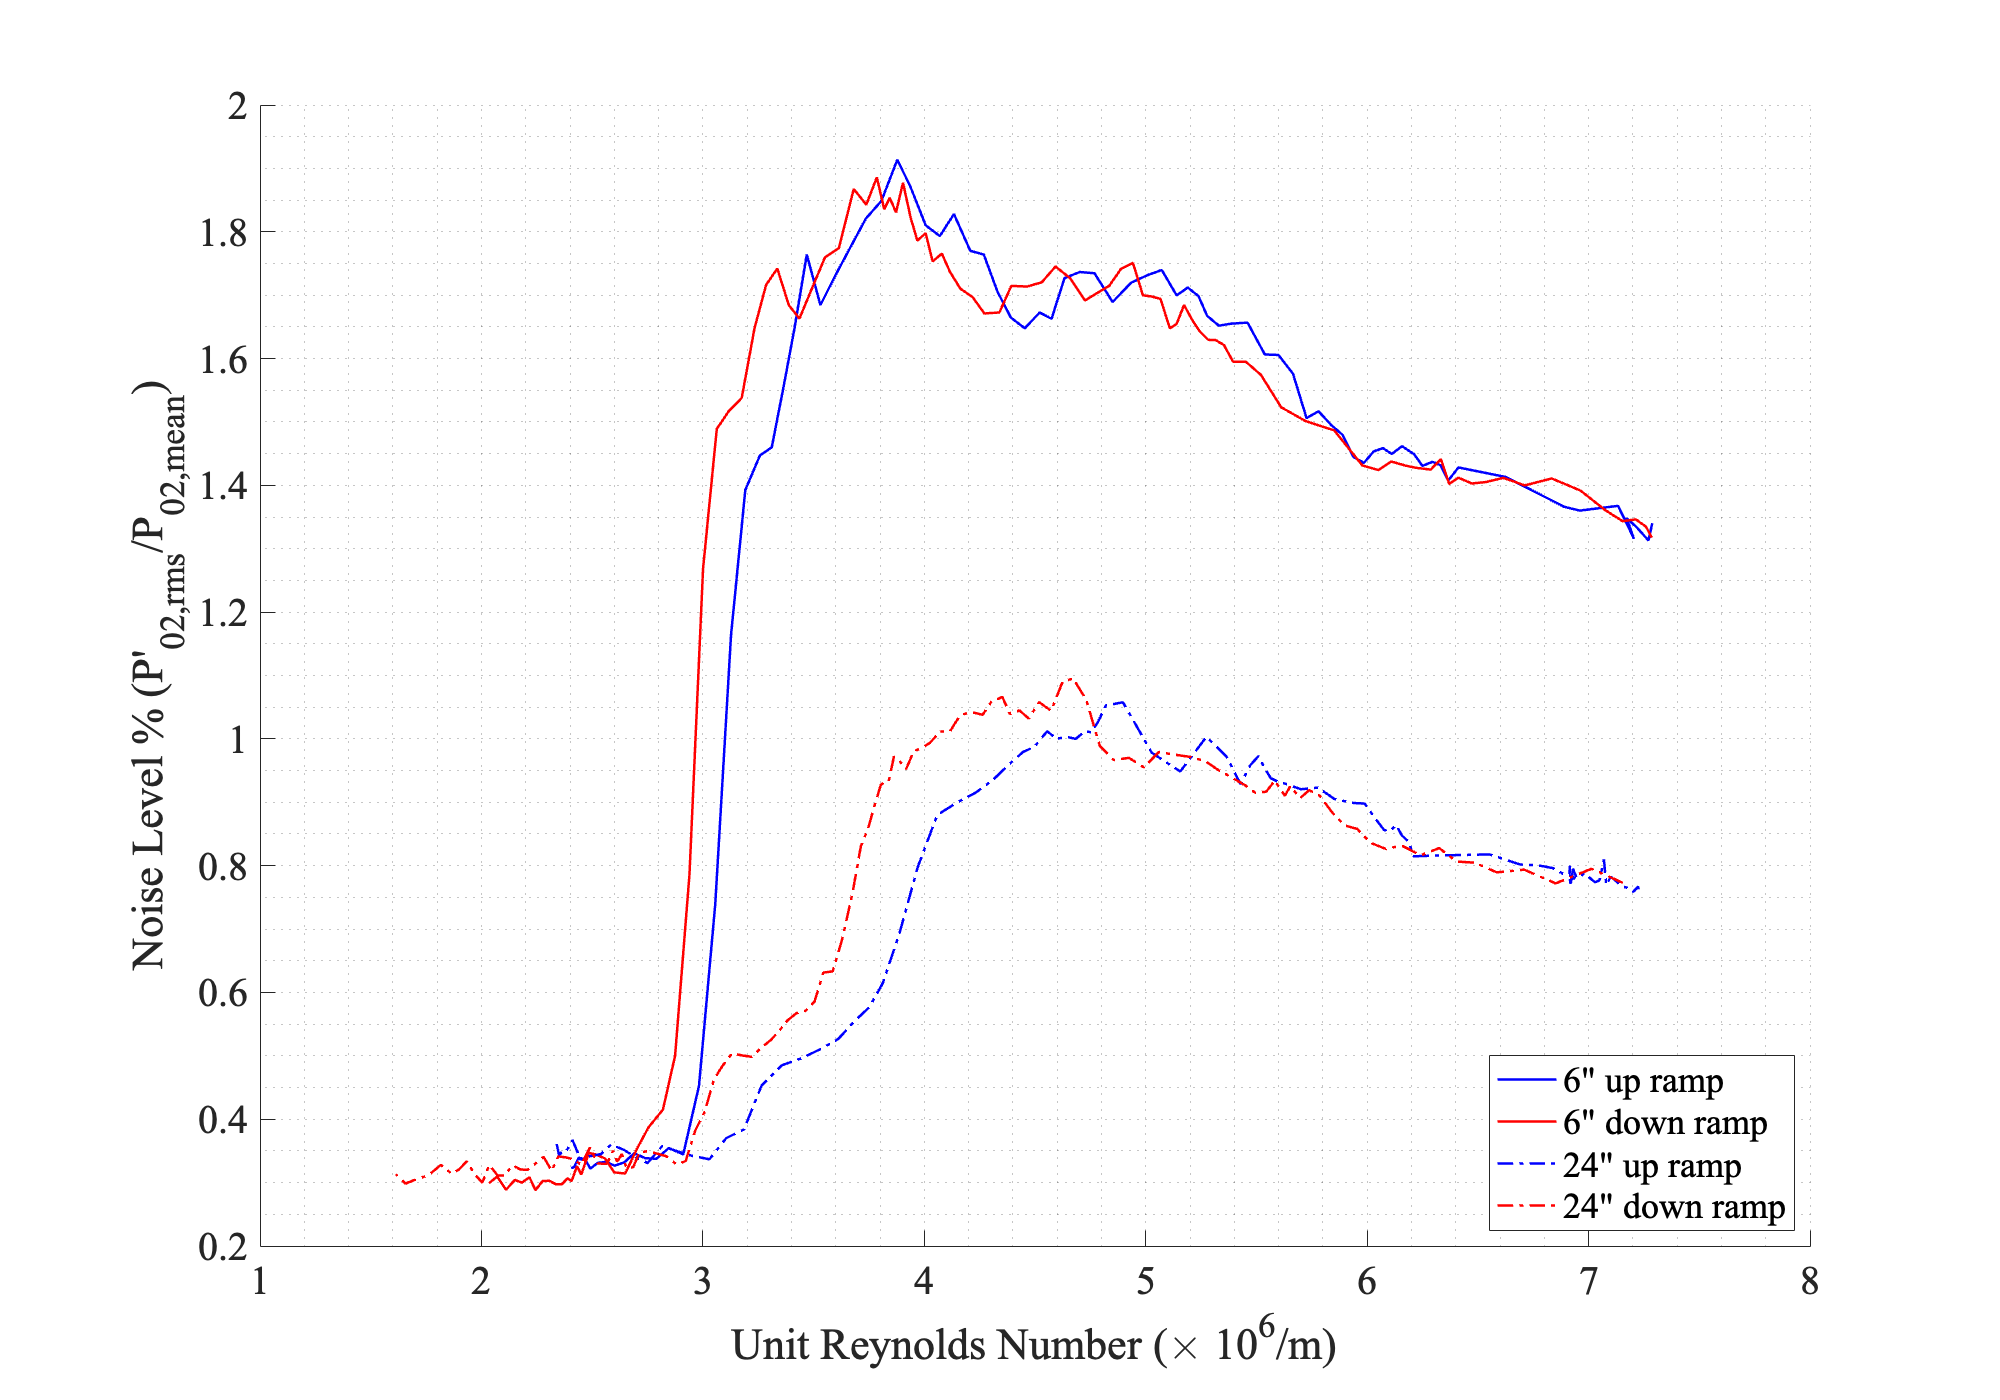
\includegraphics[width=6in]{ace-hysteresis}
    \caption{ACE freestream pressure fluctuations at 6 inches and 24 inches upstream of nozzle exit}
    \label{fig:ace-hysteresis}
\end{figure}

The anticipated characterization test matrix for ACE2.0 is shown in Table \ref{tab:ace2-survey}. The pitot rake will be used to characterize the freestream flow uniformity in the nozzle exit plane and a plane 6 inches upstream. The single pitot probe and hot-wire anemometer will be used to measure the freestream pressure fluctuation and mass flux fluctuation levels, respectively, along the centerline up to 24 inches upstream of the nozzle exit. The runs in each test matrix are divided into a few distinct objectives: (1) uniformity, (2) uncertainty quantification, (3) disturbance levels transition, and (4) hysteresis. The last five runs will be replicates of the first five to better quantify the uncertainty in Mach number, Reynolds number, and flow uniformity. This entire process will be documented so that flow-quality verification tests can be repeated as part of ongoing lab operations.

\begin{figure}[ht!]
    \centering
    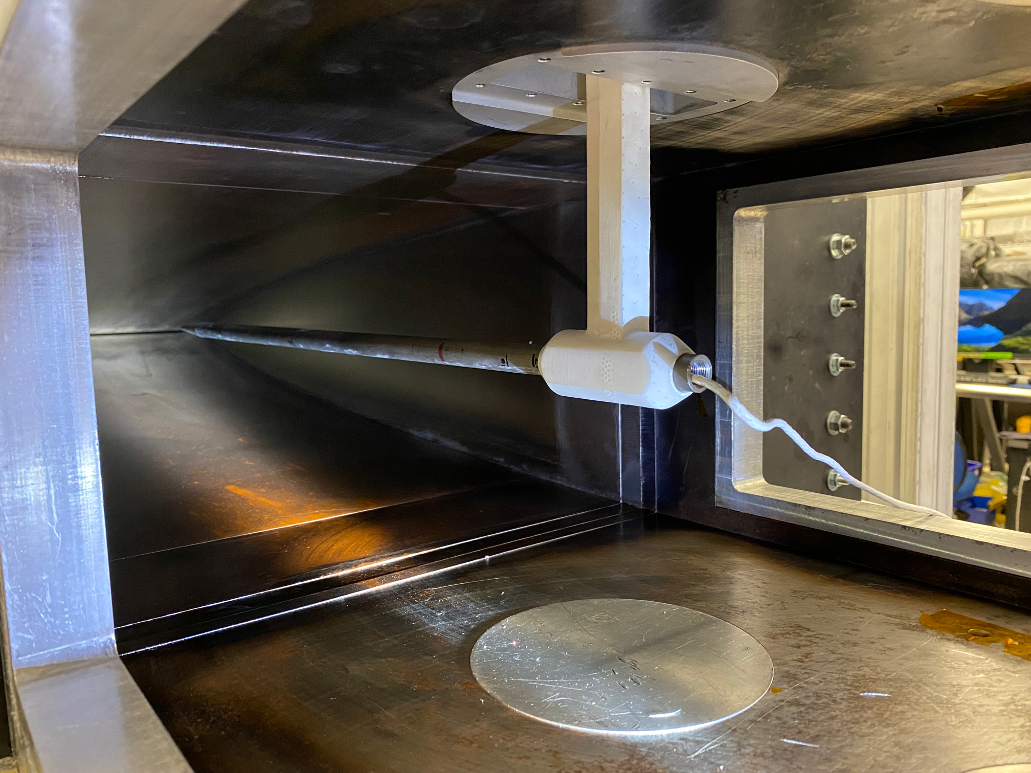
\includegraphics[width=6in]{pitot17}
    \caption{Pitot probe measuring 24 inches upstream of nozzle exit}
    \label{fig:pitot17}
\end{figure}

\setcounter{rownum}{0}
\begin{table}[ht!]
    \centering
    \begin{tabular}{|>{\stepcounter{rownum}\therownum}c|c|c|c|c|c|c|c|}
        \hline
        \multicolumn{1}{|c|}{\textbf{Run}} & \textbf{X (in.)} & \textbf{Y (in.)} & \textbf{Z (in.)} & \textbf{Mach} & $\boldsymbol{Re' \, (10^6)}$ & \textbf{ Instrument} & \textbf{Purpose} \\ \hline
        & 0 & -3:1:3 & 0 & 6 & 2$\to$10$\to$2 & Rake & Baseline\\ \hline
        & 0 & -3:1:3 & 0 & 5$\to$8$\to$5 & TBD & Rake & Baseline\\ \hline
        & 0 & -3:1:3 & -3:1:3 & 8 & TBD & Rake & Uniformity\\ \hline
        & 0 & -3:1:3 & -3:1:3 & 7 & TBD & Rake & Uniformity\\ \hline
        & 0 & -3:1:3 & -3:1:3 & 6 & TBD & Rake & Uniformity\\ \hline
        & 0 & -3:1:3 & -3:1:3 & 5 & TBD & Rake & Uniformity\\ \hline
        & -6 & -3:1:3 & -3:1:3 & 5 & TBD & Rake & Uniformity\\ \hline
        & -6 & -3:1:3 & -3:1:3 & 6 & TBD & Rake & Uniformity\\ \hline
        & -6 & -3:1:3 & -3:1:3 & 7 & TBD & Rake & Uniformity\\ \hline
        & -6 & -3:1:3 & -3:1:3 & 8 & TBD & Rake & Uniformity\\ \hline
        & 0 & 0 & 0 & 8 & 2$\to$TBD$\to$2 & Pitot & Noise\\ \hline
        & 0 & 0 & 0 & 7 & 2$\to$TBD$\to$2 & Pitot & Noise\\ \hline
        & 0 & 0 & 0 & 6 & 2$\to$TBD$\to$2 & Pitot & Noise\\ \hline
        & 0 & 0 & 0 & 5 & 2$\to$TBD$\to$2 & Pitot & Noise\\ \hline
        & 0 & 0 & 0 & 5$\to$8$\to$5 & TBD & Pitot & Noise\\ \hline
        & -6 & 0 & 0 & 5$\to$8$\to$5 & TBD & Pitot & Noise\\ \hline
        & -6 & 0 & 0 & 5 & 2$\to$TBD$\to$2 & Pitot & Noise\\ \hline
        & -6 & 0 & 0 & 6 & 2$\to$TBD$\to$2 & Pitot & Noise\\ \hline
        & -6 & 0 & 0 & 7 & 2$\to$TBD$\to$2 & Pitot & Noise\\ \hline
        & -6 & 0 & 0 & 8 & 2$\to$TBD$\to$2 & Pitot & Noise\\ \hline
        & -17 & 0 & 0 & 6 & 2$\to$TBD$\to$2 & Pitot & Noise\\ \hline
        & -17 & 0 & 0 & 5$\to$8$\to$5 & TBD & Pitot & Noise\\ \hline
        & -24 & 0 & 0 & 5$\to$8$\to$5 & TBD & Pitot & Noise\\ \hline
        & -24 & 0 & 0 & 6 & 2$\to$TBD$\to$2 & Pitot & Noise\\ \hline
        -\stepcounter{rownum}\stepcounter{rownum}\stepcounter{rownum}\stepcounter{rownum}\stepcounter{rownum}\stepcounter{rownum}\stepcounter{rownum}\therownum & \multicolumn{6}{|c|}{\textbf{Repeat a few key runs from 11-24 with Hot-wire}} & Noise\\ \hline
        -\stepcounter{rownum}\stepcounter{rownum}\stepcounter{rownum}\stepcounter{rownum}\stepcounter{rownum}\therownum & \multicolumn{6}{|c|}{\textbf{Replicate runs 1-6}} & Uncertainty\\ \hline
    \end{tabular}
    \caption{Test matrix for ACE2.0 freestream characterization.}
    \label{tab:ace2-survey}
\end{table}

\subsection{Freestream Uncertainty Quantification}

The process to quantify the uncertainty of the various parameters for this work will closely follow Stephens's et al. \cite{stephens-hubbard} and Curriston's \cite{curriston-dis} approaches by simply focusing on establishing a baseline for the uncertainty and making recommendations for improvement if necessary. The three steps to establish this baseline uncertainty for ACE2.0 will be (1) gather/measure systematic elemental uncertainties, (2) input into a Monte Carlo code along with data reduction equations to simulate systematic uncertainties, and (3) measure repeat data points through a few replicate experiments and calculate random uncertainties.

First, the systematic elemental uncertainties can be gathered and measured from the various sensors, which includes the static pressure transducer, stagnation pressure transducer, stagnation temperature thermocouple, and servo motor internal encoders. Each of these has a predefined manufacturer uncertainty that can be used, but some of these are very conservative and not ideal. The pressure sensors and temperature sensor will be tested against a working standard to measure the true uncertainty, which is often found to be an order of magnitude less than the manufacturer uncertainty \cite{curriston-dis}. The systematic uncertainly of any sensors utilized in future experiments is outside the scope of this work and must be considered when calculating the total uncertainty of measurements in each experiment.

Next, these systematic elemental uncertainties will be propagated through a Monte Carlo simulation along with the specific data reduction equations for the facility. This output will provide the total systematic uncertainty for each parameter of interest, which will be added to the random uncertainty to give the total uncertainty. Additionally, this simulation will also be used provide a sensitivity analysis of the uncertainty to the various input parameters. This will be insightful on how to best improve the uncertainty if necessary.

Finally, repeat data points will be measured by repeatedly settling on and off the set condition for the parameter of interest. While data will be gathered throughout the entire characterization test matrix, runs 1 and 20 will be solely for repeat data measurements. These two runs will provide a direct comparison of replicates that will account for any correlations that were not considered or unquantifiable. The standard deviation of this data will be added in quadrature to the systematic uncertainty to calculate the total uncertainty for each parameter of interest for the freestream flow.

\subsection{Freestream Disturbance Hysteresis}

Dynamic sweeps of both Mach number and Reynolds number will be performed to explore any potential hysteresis effects in either the noise or the control parameters. Specifically, this will be accomplished during the dynamic runs in the characterization test matrix in Table \ref{tab:ace2-survey}. The goal is simply to identify the existence of any hysteresis effects to inform future work within ACE2.0. The Reynolds number sweep runs are necessary to determine the value at which transition occurs, so sweeping the Reynolds number back down will not add any additional work and will be ensure that there is no hysteresis. For the Mach number however, there is no past data to determine the existence of hysteresis, so these runs will establish a baseline. The noise level is known to decrease with an increase in Mach number, so identifying any hysteresis in this will be necessary to inform future experiments.

\section{Mach Trajectory and Potential Hysteresis Proof of Concept Experiment}

This objective will primarily serve as a demonstration of the capabilities for ACE2.0 and will also provide preliminary insight into the hysteretic behavior of dynamic Mach number experiments. The flow characteristic that will be specifically explored in this research will be shock interactions using schlieren. The goal will be to observe hysteresis in the transition from regular reflection to Mach reflection by varying the Mach number. The challenge of this is that the only facilities that have successfully produced this hysteresis had low freestream disturbance levels and an open-jet test section, while ACE2.0 has a closed test section and is not considered a "quiet" facility. In order to provide the best conditions for hysteresis to be observed, these experiments will be performed at higher Mach numbers and a lower unit Reynolds number where freestream disturbance levels are lowest.

The experiments will be based on the methodologies and results from Durand et al. \cite{durand} and Tao et al. \cite{tao} in addition to the experimental setup of Mai \cite{mai-dis}. The Mach number will be varied across either the Von Neumann condition or the detachments criteria to force the transition from regular reflection to Mach reflection or vice versa. In order to choose the wedge angle and Mach number range for each experiment, Figure \ref{fig:dual} was created following the processes shown by Mouton \cite{mouton} for each condition. Using the pressure ratio and flow deflection angle for an oblique shock, the shock angle is solved numerically as a function of the freestream Mach number for each condition. The shock angle and Mach number are then used to produce the detachment and Von Neumann condition relationship between wedge angle and Mach number. Below the Von Neumann condition, only regular reflections are possible as shown in Figure \ref{fig:von-neumann}. Above the detachment condition, only Mach reflections are possible as shown in Figure \ref{fig:detachment}. Between these two condition, either shock formation is possible.

% The basic parameters across an oblique shock shown in Figure \ref{fig:detachment} are given as a function of the Mach number in region x $\left(M_x\right)$, the shock angle ($\alpha$), and the ratio of specific heats ($\gamma$). 

% The pressure ratio is 
% \begin{equation}
%     \xi \left(M_x,\alpha\right) = \frac{P}{P_x} = \frac{2 \gamma M_x^2 \sin^2{\alpha} - (\gamma-1)}{\gamma+1}
% \end{equation}

% \noindent The flow deflection angle (wedge angle) and Mach number are given as
% \begin{equation}
%     \theta \left(M_x,\alpha\right) = \cot^{-1}{\left[ \left(\frac{(\gamma+1) M_x^2}{2\left(M_x^2 \sin^2{\alpha} - 1\right)}\right) \tan{\alpha} \right]}
% \end{equation}
% \begin{equation}
%     M \left(M_x,\alpha\right) = \sqrt{\frac{(\gamma+1)^2 M_x^4 \sin^2{\alpha} - 4\left(M_x^2 \sin^2{\alpha} - 1\right)\left(\gamma M_x^2 \sin^2{\alpha} + 1\right)}{\left[2 \gamma M_x^2 \sin^2{\alpha} - (\gamma-1)\right]\left[(\gamma-1) M_x^2 \sin^2{\alpha} + 2\right]}}
% \end{equation}

% The shock angle when the flow deflection angle is maximum is given by setting $\frac{\partial \theta}{\partial \alpha} = 0$, resulting in
% \begin{equation}
%     \alpha^{\theta_{max}}(M_x) = \sin^{-1}{\sqrt{(\gamma+1)\frac{M_x^2 - \frac{4}{\gamma+1} + \sqrt{M_x^4 + 8\frac{\gamma-1}{\gamma+1}M_x^2 + \frac{16}{\gamma+1}}}{4 \gamma M_x^2}}}
% \end{equation}

% For the detachment condition shown in Figure \ref{fig:detachment}
% \begin{equation}
%     M_{1,D} = M(M_{\infty},\alpha_D)
% \end{equation}
% \begin{equation}
%     \theta(M_{\infty},\alpha_D) = \theta\left(M_{1,D},\alpha^{\theta_{max}}(M_{1,D})\right)
% \end{equation}

% Solving this for $\alpha_D$ results in a fifth-order polynomial in $\sin^2{\alpha_D}$
% \begin{equation}
%     D_0 + D_1 \sin^2{\alpha_D} + D_2 \sin^4{\alpha_D} + D_3 \sin^6{\alpha_D} + D_4 \sin^8{\alpha_D} + D_5 \sin^{10}{\alpha_D} = 0
% \end{equation}

% where
% \begin{align*}
%     D_0 =& -16 \\
%     D_1 =& \; 32M_{\infty}^2 - 4M_{\infty}^4 - 48M_{\infty}^2\gamma - 16M_{\infty}^4\gamma + 16\gamma^2 - 16M_{\infty}^4\gamma^2 \\
%          & + 16M_{\infty}^2\gamma^3 + 4M_{\infty}^4\gamma^4 \\
%     D_2 =& - 16M_{\infty}^4 + 4M_{\infty}^6 - M_{\infty}^8 + 104M_{\infty}^4\gamma + 16M_{\infty}^6\gamma - 4M_{\infty}^8\gamma \\
%          & - 64M_{\infty}^2\gamma^2 - 32M_{\infty}^4\gamma^2 + 8M_{\infty}^6\gamma^2 - 6M_{\infty}^8\gamma^2 -56M_{\infty}^4\gamma^3 \\
%          & - 16M_{\infty}^6\gamma^3 - 4M_{\infty}^8\gamma^3 - 12M_{\infty}^6\gamma^4 - M_{\infty}^8\gamma^4 \\
%     D_3 =& \; M_{\infty}^8 - 64M_{\infty}^6\gamma + 4M_{\infty}^8\gamma + 96M_{\infty}^4\gamma^2 +64M_{\infty}^6\gamma^2 + 14M_{\infty}^8\gamma^2 \\
%          & + 64M_{\infty}^6\gamma^3 +20M_{\infty}^8\gamma^3 + 9M_{\infty}^8\gamma^4 \\
%     D_4 =& \; 8M_{\infty}^8\gamma - 64M_{\infty}^6\gamma^2 - 32M_{\infty}^8\gamma^2 - 24M_{\infty}^8\gamma^3 \\
%     D_5 =& \; 16M_{\infty}^8\gamma^2 \\
% \end{align*}

% This equation is solved numerically for Mach numbers greater than unity, and only one solution for each $\sin^{2}{\alpha_D}$ exists that is real and bounded between zero and one. The values of $\theta_D(M) = \theta\left(M_{\infty},\alpha_D\right)$ solved for freestream Mach numbers from 2 to 9 yields the upper curve in Figure \ref{fig:dual}.

% For the Von Neumann condition shown in Figure \ref{fig:von-neumann}
% \begin{equation}
%     M_{1,V} = M(M_{\infty},\alpha_V)
% \end{equation}
% \begin{equation}
%     \xi\left(M_{\infty},\frac{\pi}{2}\right) = \xi\left(M_{\infty},\alpha_V\right) \xi\left(M_{1,V},\alpha_{1,V}\right)
% \end{equation}
% \begin{equation}
%     \frac{2 \gamma M_{1,V}^2 \sin^2{\alpha_{1,V}} - (\gamma-1)}{\gamma+1} = \frac{\xi\left(M_{\infty},\frac{\pi}{2}\right)}{\xi\left(M_{\infty},\alpha_V\right)}
% \end{equation}
% \begin{equation}
%     \alpha_{1,V} = \sin^{-1}{\sqrt{\frac{(\gamma-1)+(\gamma+1)\frac{\xi\left(M_{\infty},\frac{\pi}{2}\right)}{\xi\left(M_{\infty},\alpha_V\right)}}{2 \gamma M_{1,V}^2}}}
% \end{equation}

% The solution for $\alpha_{1,V}$ is found numerically by solving the equation
% \begin{equation}
%     \theta\left(M_{\infty},\alpha_V\right) = \theta\left(M_{1,V},\alpha_{1,V}\right) 
% \end{equation}

% The values of $\theta_V(M) = \theta\left(M_{\infty},\alpha_V\right)$ solved for freestream Mach numbers from 2.2 to 9 yields the lower curve in Figure \ref{fig:dual}.

\begin{figure}[ht!]
    \centering
    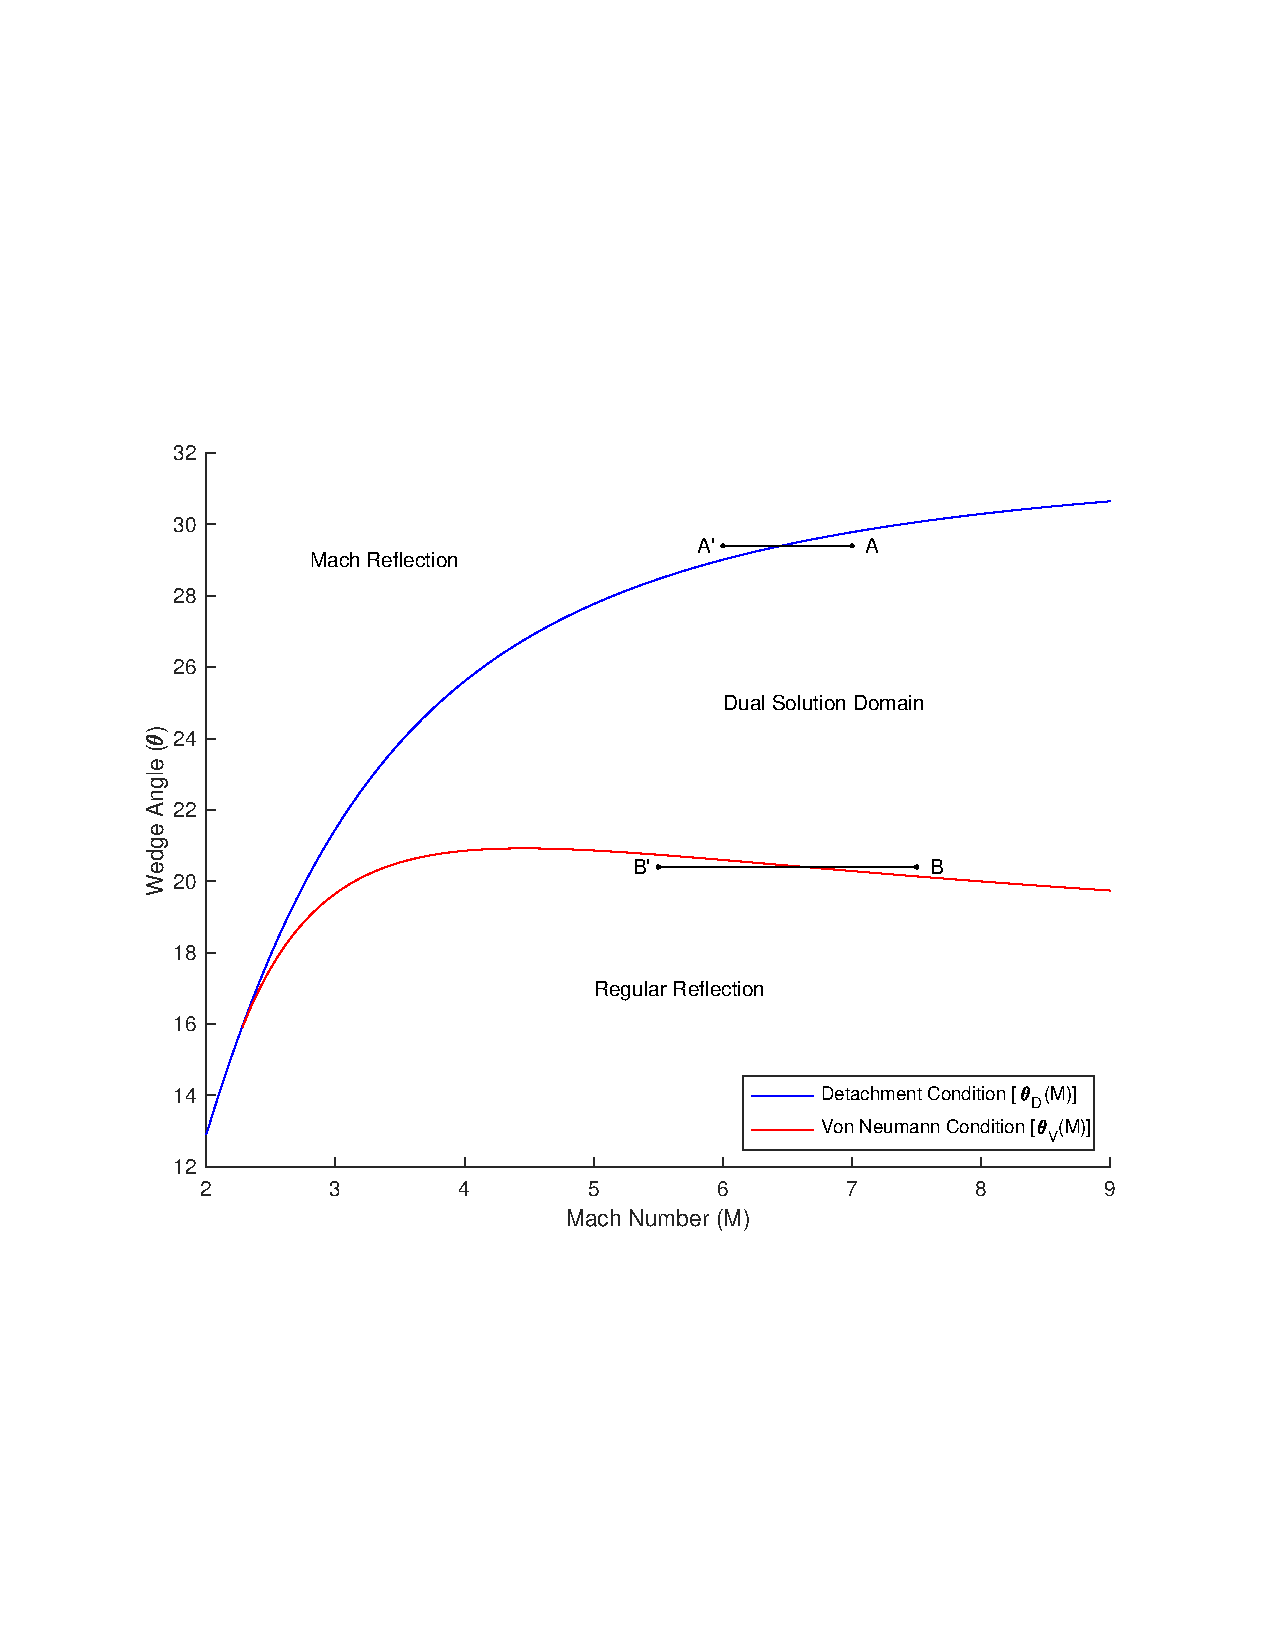
\includegraphics[trim={70 200 70 200},clip,width=6in]{dual.pdf}
    \caption{Shock wave reflection configuration domains for Mach number and wedge angle}
    \label{fig:dual}
\end{figure}

\begin{figure}[ht!]
    \centering
    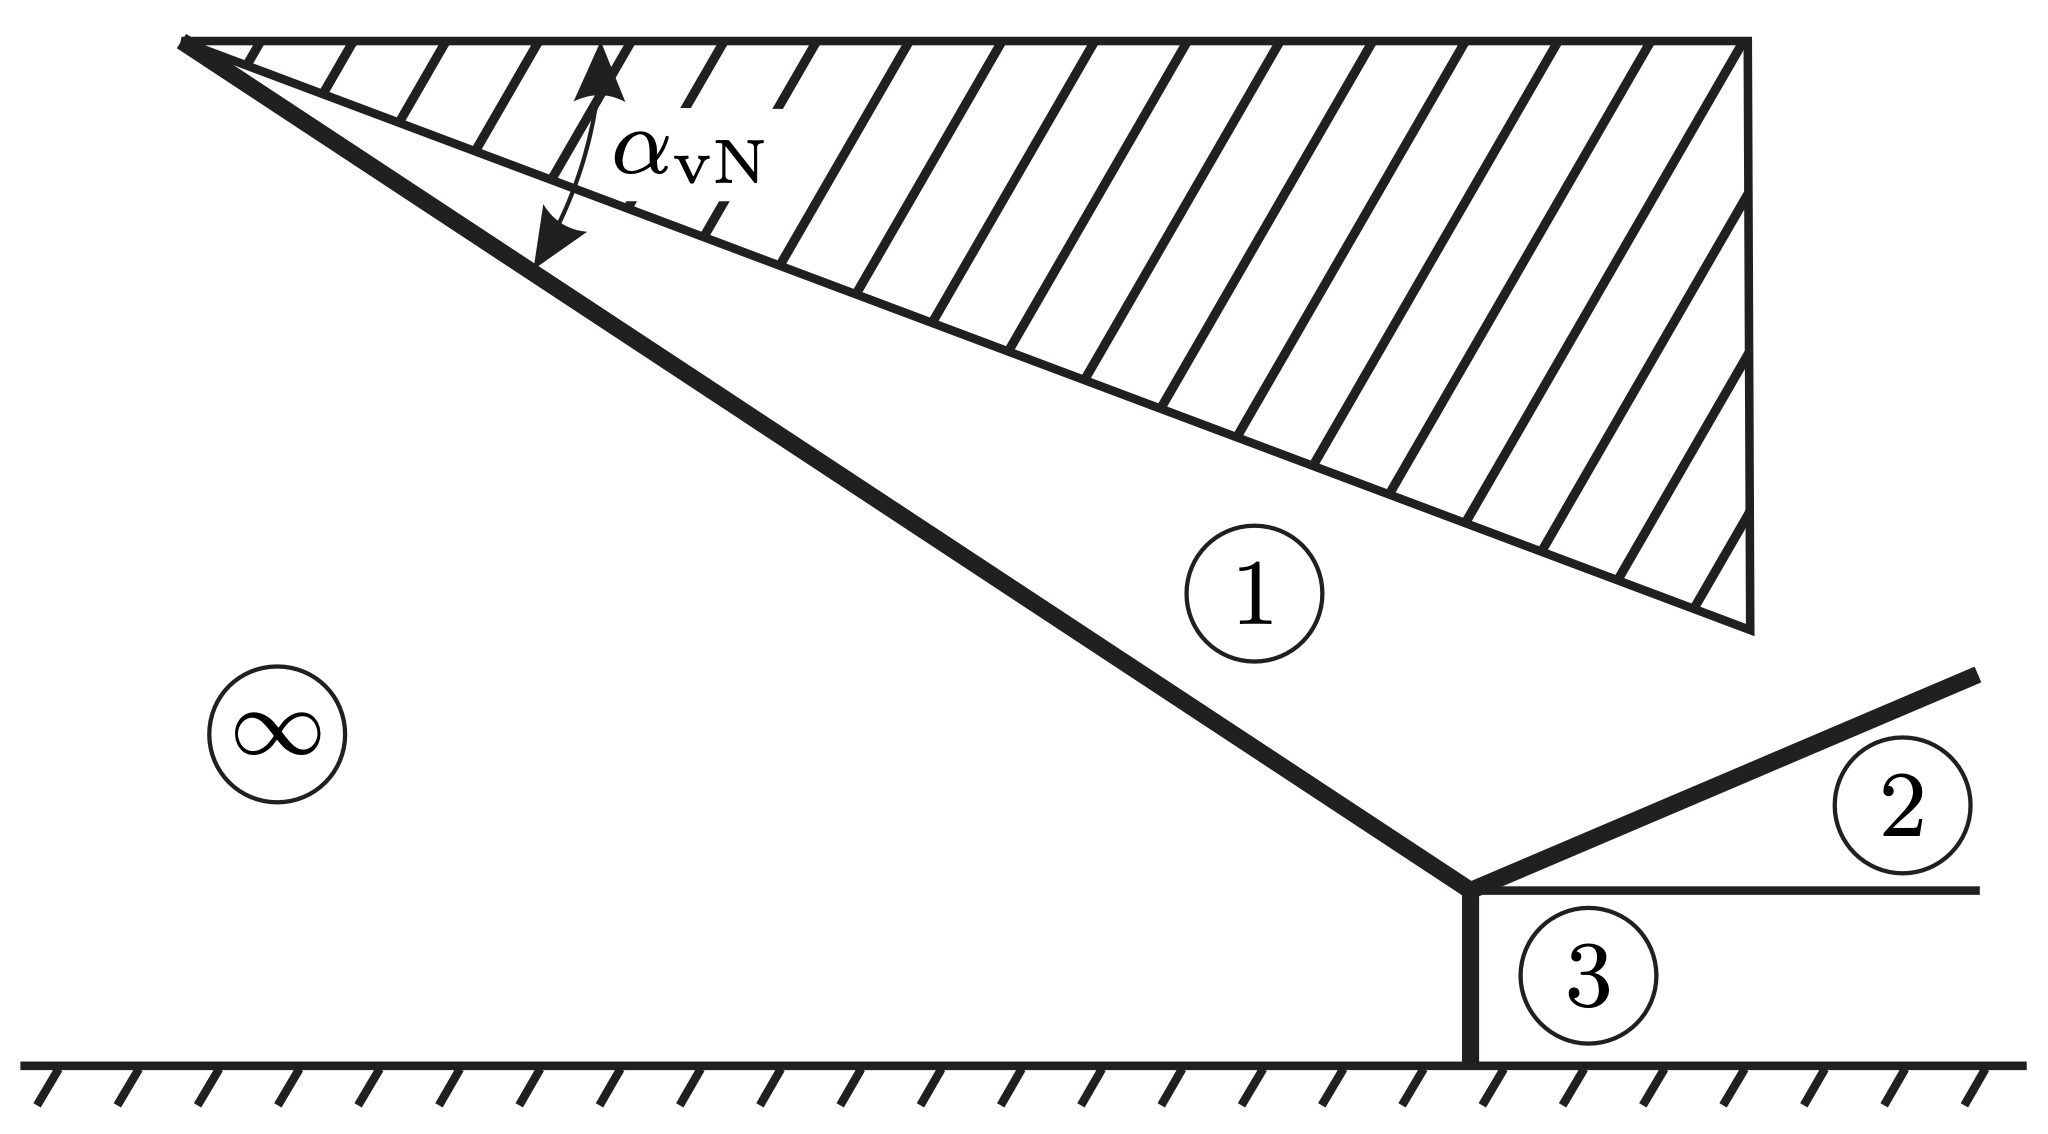
\includegraphics[width=4in]{von-neumann}
    \caption[Flow over wedge resulting in Mach reflection of shock]{Flow over wedge resulting in Mach reflection of shock \cite{mouton}}
    \label{fig:von-neumann}
\end{figure}

\begin{figure}[ht!]
    \centering
    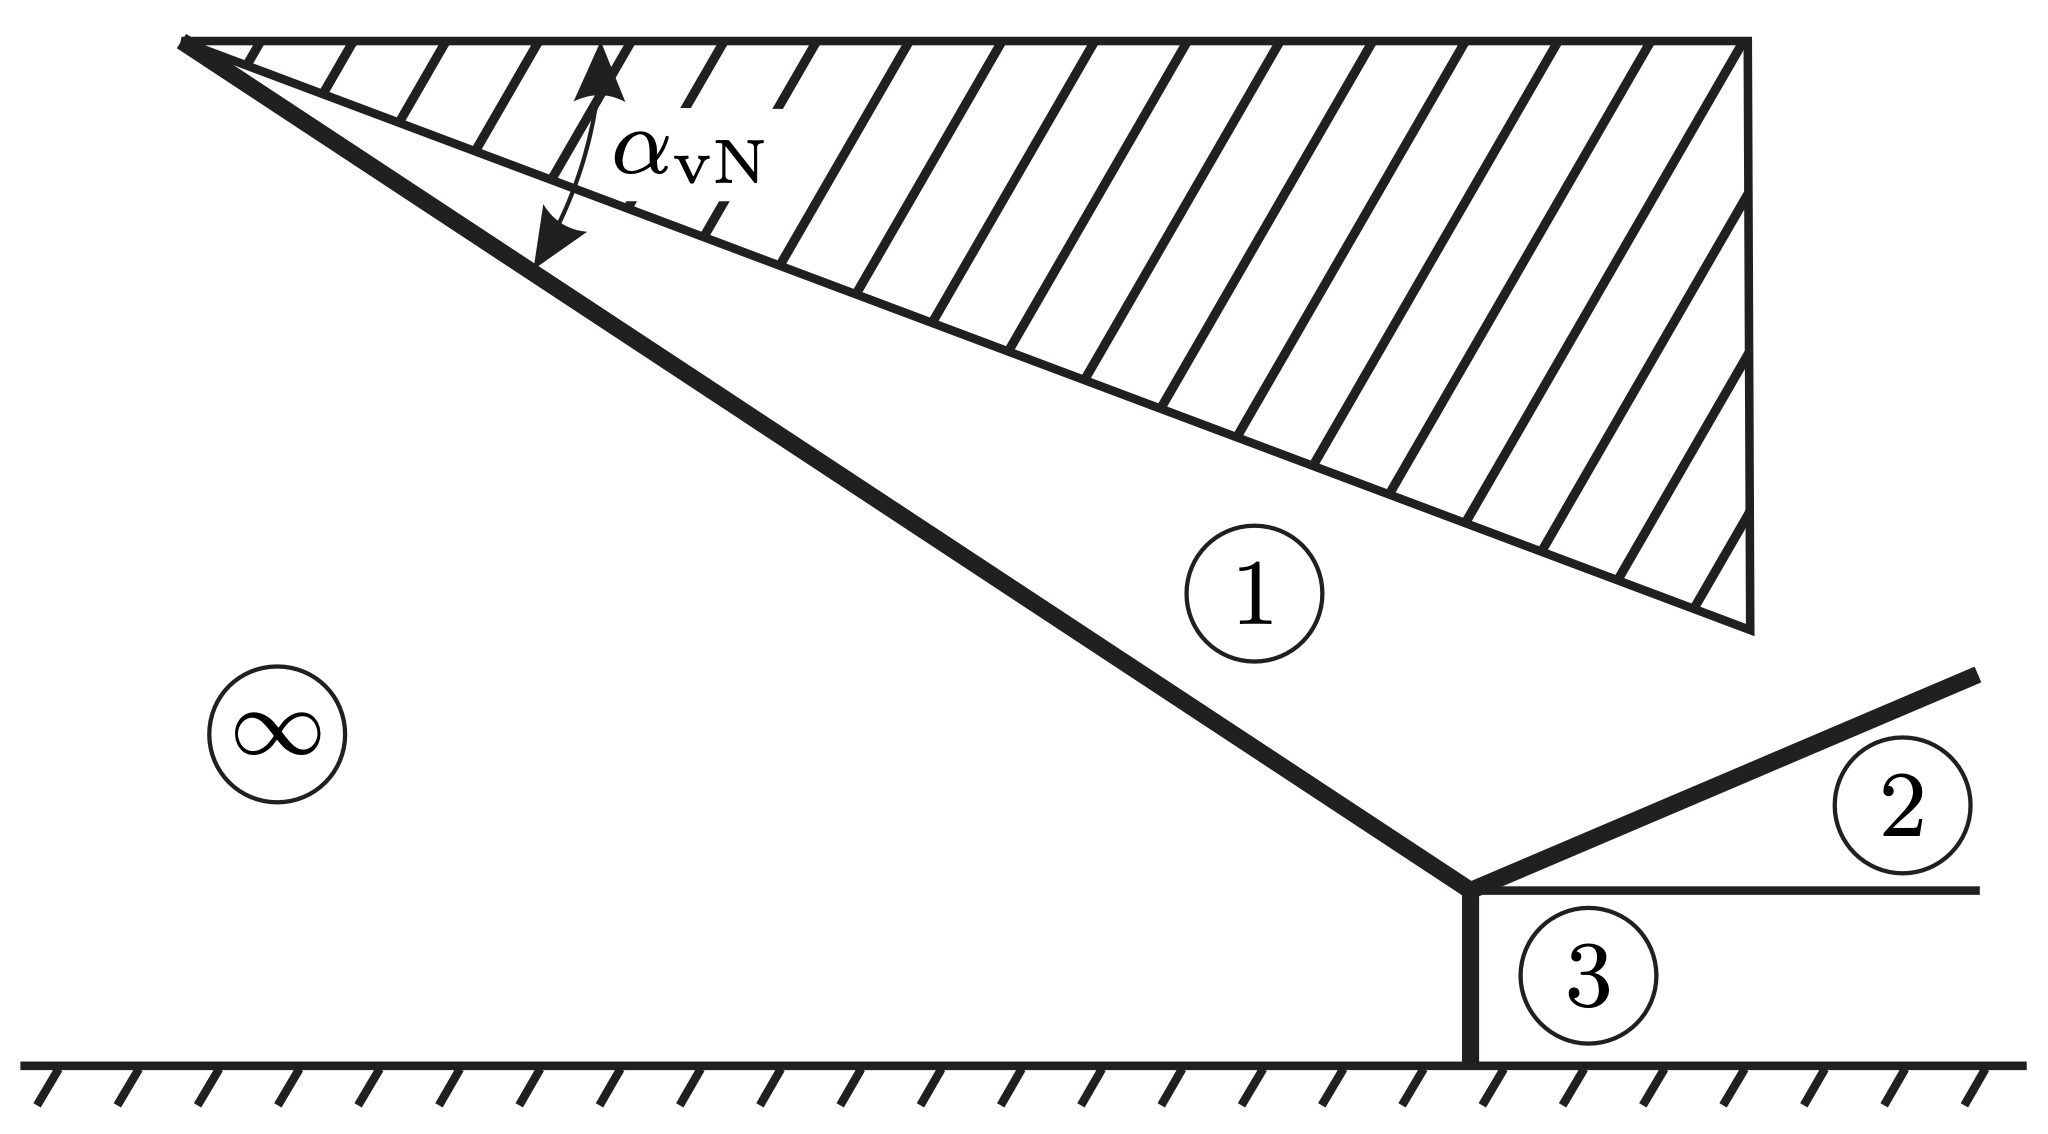
\includegraphics[width=4in]{detachment}
    \caption[Flow over wedge resulting in regular reflection of shock]{Flow over wedge resulting in regular reflection of shock \cite{mouton}}
    \label{fig:detachment}
\end{figure}

The two experimental setups are shown as A and B in Figure \ref{fig:dual}. For A, the wedge angle is 30$\degree$ and the Mach number range is 7 to 8. For B, the wedge angle is 20.3$\degree$ and the Mach number range is 6 to 8. For both paths, the Mach number will start at the point in the dual solution domain, decrease across either the detachment condition or the Von Neumann condition, and then increase back into the dual solution domain (i.e. AA'A, BB'B). The reverse of these will also be explored if hysteresis is not observed initially.

The physical model for these experiments will be very similar to the double wedge setup used by Mai \cite{mai-dis} in ACE as shown in Figure \ref{fig:wedges}. If 3D printing with Rigid 10K produces an acceptable leading edge, then a pair will be printed for each angle needed. If future research will utilize this double wedge setup, then a hinged mechanism will be designed and fabricated to use a single pair of wedges for any desired angle.

\begin{figure}[ht!]
    \centering
    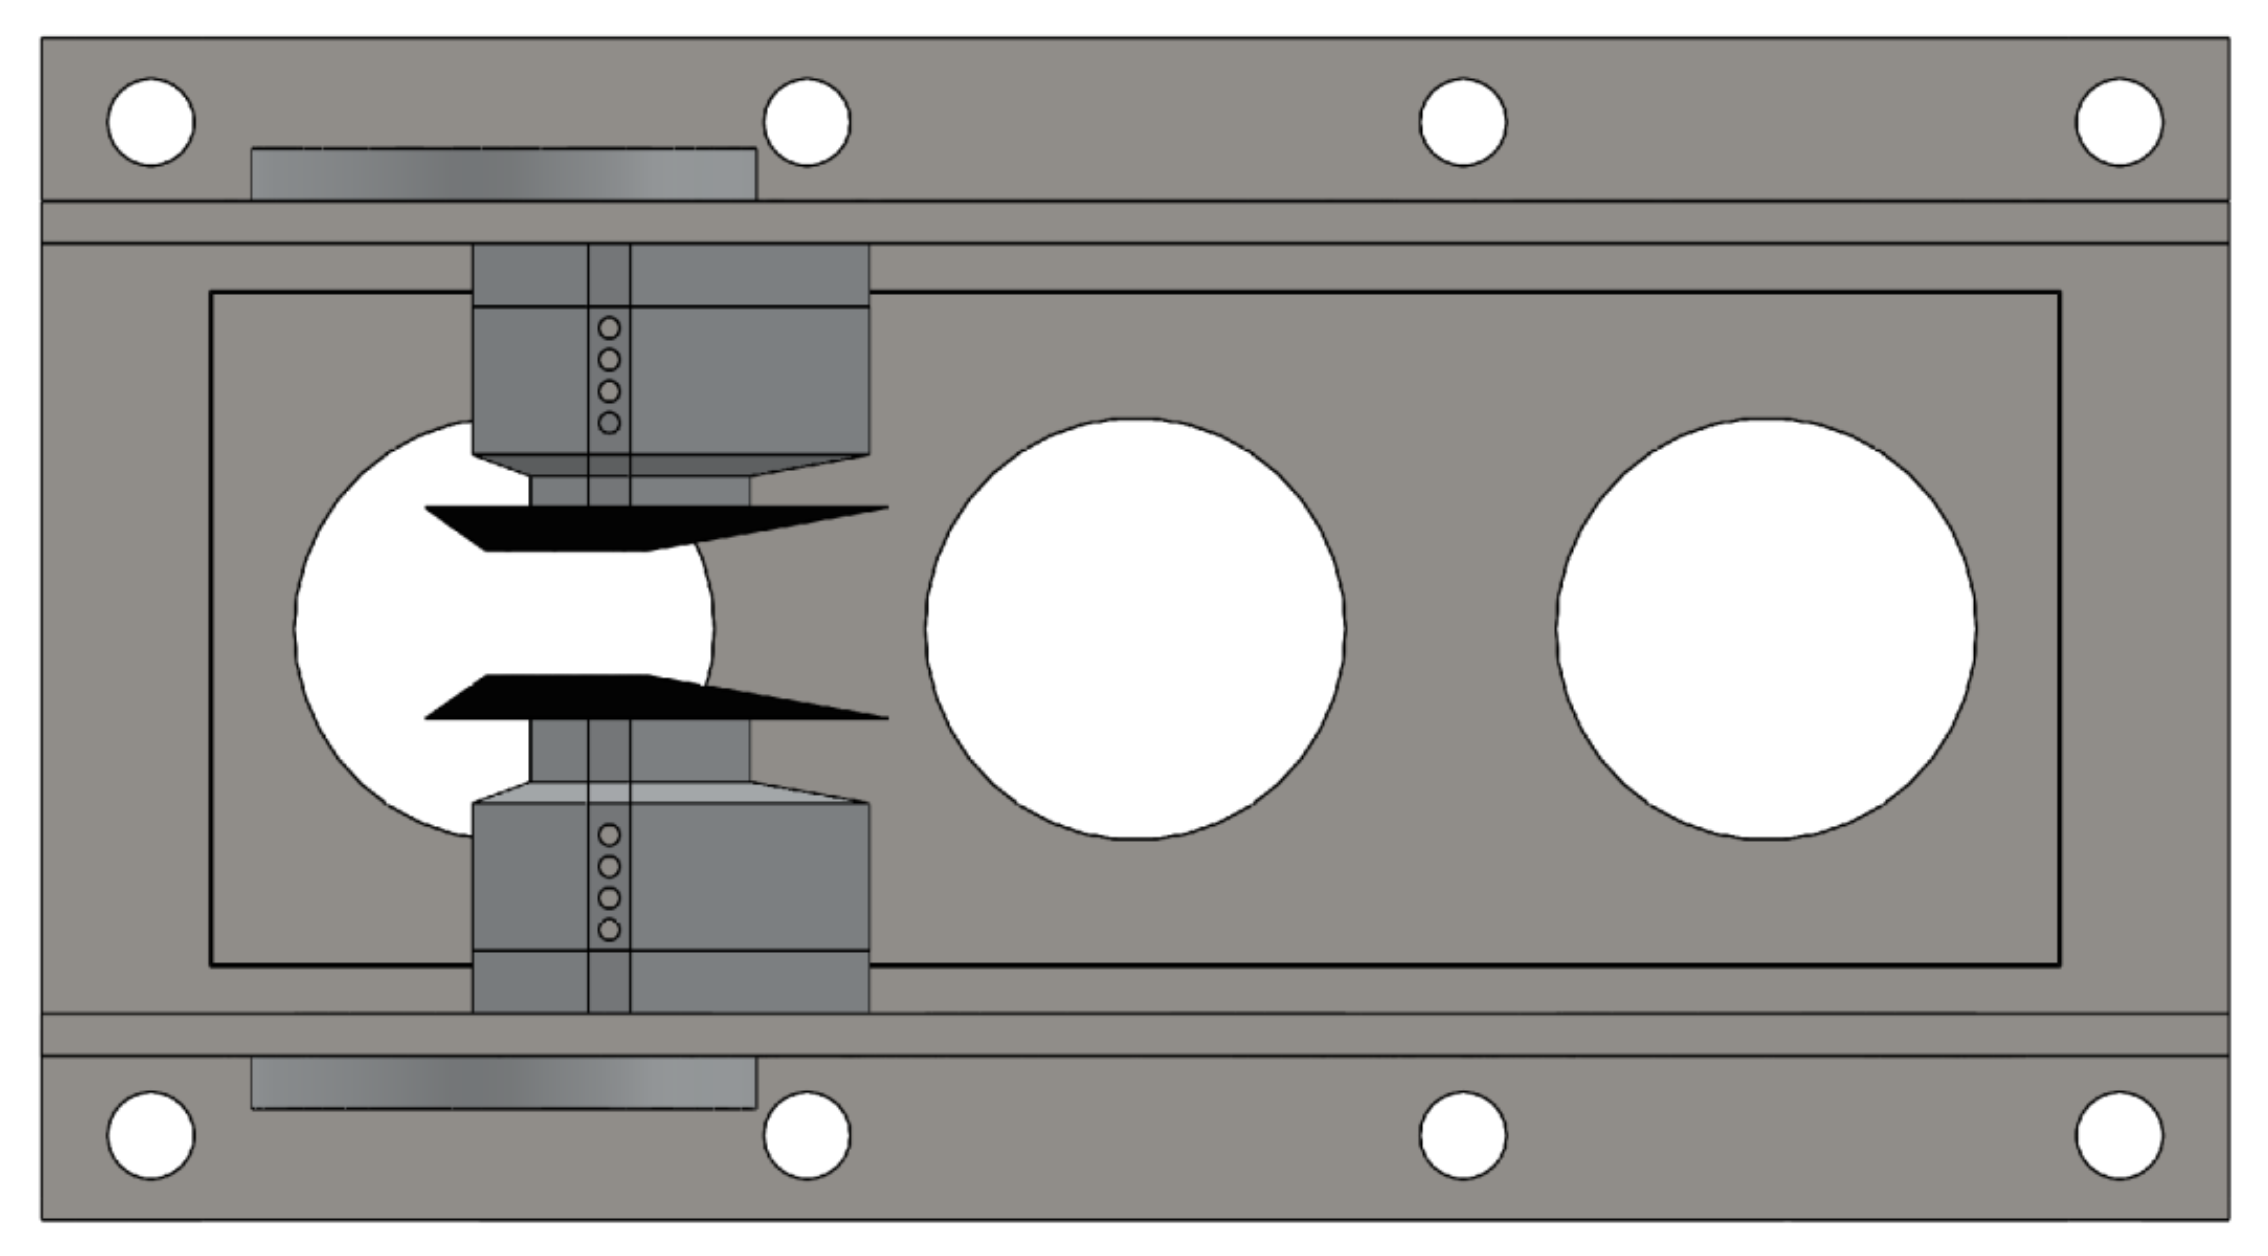
\includegraphics[width=6in]{wedges}
    \caption[Double wedge experiment setup]{Double wedge experiment setup \cite{mai-dis}}
    \label{fig:wedges}
\end{figure}

The expected results should appear similar to the numerical results from Ben-Dor et al. \cite{ben-dor-1}, Durand et al. \cite{durand}, and Tao et al. \cite{tao} with an example shown in Figure \ref{fig:shock-hysteresis}. Although the Mach number range and wedge angle are different, the hysteresis should be the same for the chosen paths in this experiment. The path in Figure \ref{fig:shock-hysteresis} is representative of path AA'A, which crosses the detachment condition. There have not been any simulations published that cross the Von Neumann condition by varying the Mach number, so path B will be explored secondary to path A.

In either case, the final objective will be to guide future experiments by determining if ACE2.0 is capable of reproducing the hysteresis in shock interactions or incapable due to freestream noise. 

\begin{figure}[ht!]
    \centering
    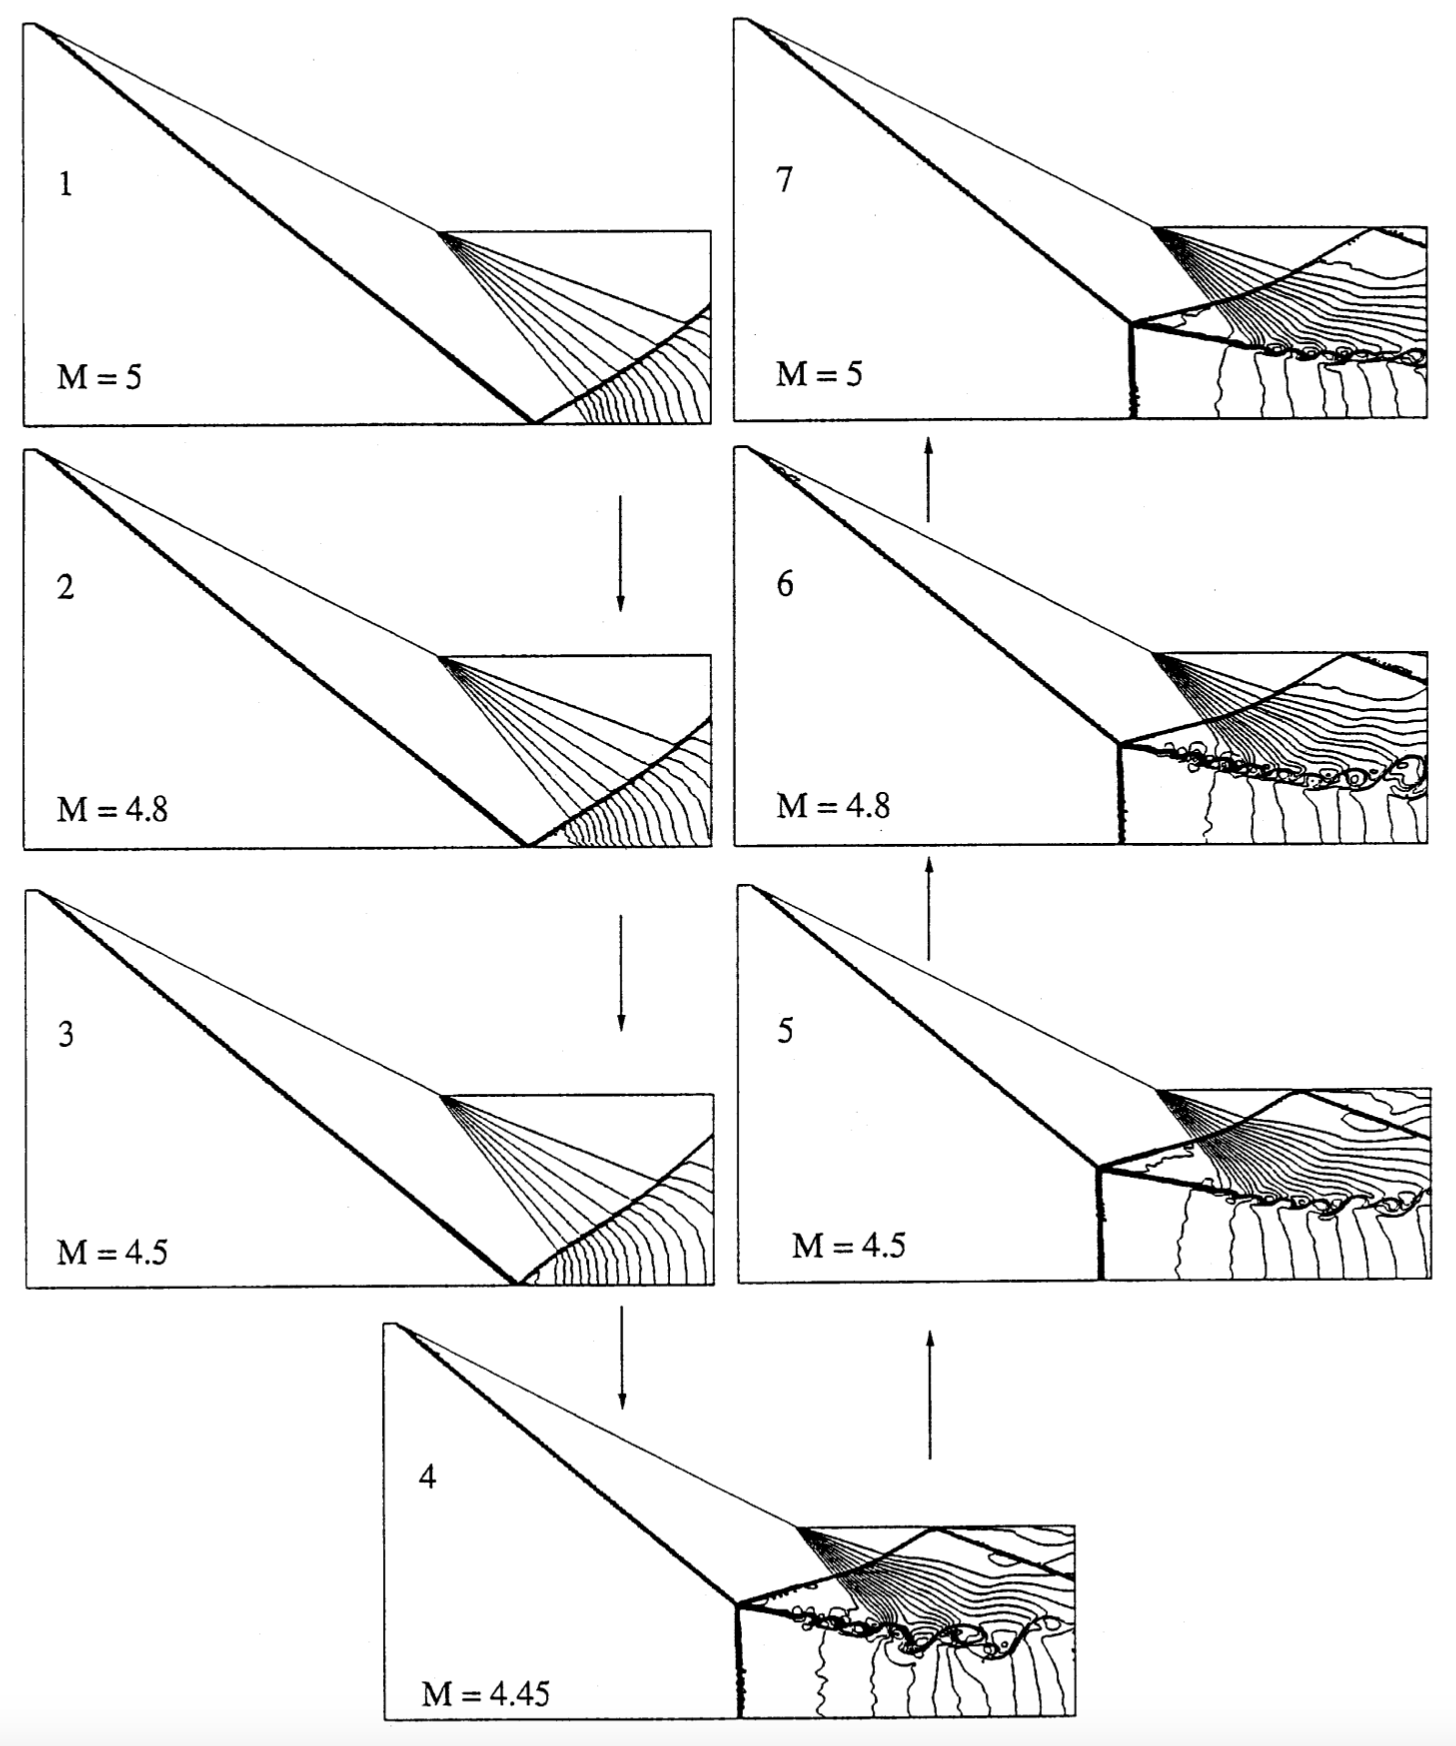
\includegraphics[width=6in]{shock-hysteresis}
    \caption[Mach-number-varitation-induced hysteresis for 27$\degree$ wedge]{Mach-number-variation-induced hysteresis for 27$\degree$ wedge \cite{ben-dor-1}}
    \label{fig:shock-hysteresis}
\end{figure}




%%%%%%%%%%%%%%%%%%%%%%%%%%%%%%%%%%%%%%%%%%%%%%%%%%%
%
%  Author: Jacob Vaughn
%  
%  Last Updated: 1/13/2024
%
%%%%%%%%%%%%%%%%%%%%%%%%%%%%%%%%%%%%%%%%%%%%%%%%%%%
%%%%%%%%%%%%%%%%%%%%%%%%%%%%%%%%%%%%%%%%%%%%%%%%%%%%%%%%%%%%%%%%%%%%%%
%%                          RESULTS
%%%%%%%%%%%%%%%%%%%%%%%%%%%%%%%%%%%%%%%%%%%%%%%%%%%%%%%%%%%%%%%%%%%%%



\chapter{RESULTS AND DISCUSSION}

Stuff about experminet results

\begin{figure}[ht]
    \centering
    
\includegraphics[width=6in]{tamulogo}
    \caption{A caption about penguins}
\end{figure}

More stuff

\section{Maybe}

\section{Possibly}

%%%%%%%%%%%%%%%%%%%%%%%%%%%%%%%%%%%%%%%%%%%%%%%%%%%
%
%  Author: Jacob Vaughn
%  
%  Last Updated: 3/8/2024
%
%%%%%%%%%%%%%%%%%%%%%%%%%%%%%%%%%%%%%%%%%%%%%%%%%%%
%%%%%%%%%%%%%%%%%%%%%%%%%%%%%%%%%%%%%%%%%%%%%%%%%%%%%%%%%%%%%%%%%%%%%%
%%                         CONCLUSIONS
%%%%%%%%%%%%%%%%%%%%%%%%%%%%%%%%%%%%%%%%%%%%%%%%%%%%%%%%%%%%%%%%%%%%%%

\chapter{CONCLUSIONS}

\section{Concluding Remarks}

The path forward will follow the manufacturing schedule shown in Figure \ref{fig:schedule}. The pressure test will be performed as soon as the nozzles are finished machining, tentatively May 1, 2024. Depending on the results of the pressure test, the process could be anywhere from a single day to two weeks. Once complete though, the nozzles and sidewalls will be shipped to the polishing vendor, which should have a quick turn around of two weeks. Upon arrival to the NAHL, the full ACE2.0 nozzle will be finally assembled and installed. With proper planning prior to the final installation, the process should not take more than a week to begin shakedown and characterization.

In the meantime, the servo control program will be written between now and the pressure test. The Mach number feedback will be implemented, and the Reynolds number control capability will be explored and potentially implemented before the final install. Again, this will primarily depend on the test schedule for the M6QT and the amount of time needed to replace the manual valve with a controlled valve. 

The characterization and hysteresis experiments will be performed immediately following installation and initial calibration. The primary goal is to ensure complete function of ACE2.0 along with a demonstration of the capabilities and potential for future research. Additionally, the documentation for the nozzle operation will be written based on the best practices deduced throughout the experiments.

\section{Impact and Future Work}

Stuff

%%%%%%%%%%%%%%%
% End of body %
%%%%%%%%%%%%%%%

\nocite{aiaa-uncertainty-standard}
\nocite{anderson-fundamentals}
\nocite{anderson-compressible}


%%%%%%%%%%%%%%%%%%%%%%%%%%%%%%%%%%%%%%%%%%%%%%%%%%%%%%%%%%%%%
\let\oldbibitem\bibitem
\renewcommand{\bibitem}{\setlength{\itemsep}{0pt}\oldbibitem}
%%%%%%%%%%%%%%%%%%%%%%%%%%%%%%%%%%%%%%%%%%%%%%%%%%%%%%%%%%%%%%%
%The bibliography style declared is the IEEE format. If
%you require a different style, see the document
%bibstyles.pdf included in this package. This file,
%hosted by the University of Vienna, shows several
%bibliography styles and examples of in-text citation
%and a references page.
\bibliographystyle{ieeetr}

\phantomsection
\addcontentsline{toc}{chapter}{REFERENCES}

\renewcommand{\bibname}{{\normalsize\rm REFERENCES}}

\bibliography{data/myReference}

% Appendices main file
%%%%%%%%%%%%%%%%%%%%%%%%%%%%%%%%%%%%%%%%%%%%%%%%%%%
%
%  New template code for TAMU Theses and Dissertations starting Spring 2021.  
%
%
%  Author: Thesis Office
%  
%  Last Updated: 1/13/2021
%
%%%%%%%%%%%%%%%%%%%%%%%%%%%%%%%%%%%%%%%%%%%%%%%%%%%

\begin{appendices}
\titleformat{\chapter}{\centering\normalsize}{APPENDIX \thechapter}{0em}{\vskip .5\baselineskip\centering}
\renewcommand{\appendixname}{APPENDIX}

%%%%%%%%%%%%%%%%%%%%%%%%%%%%%%%%%%%%%%%%%%%%%%%%%%%
%
%  New template code for TAMU Theses and Dissertations starting Spring 2021.
%
%
%  Author: Thesis Office 
%	 
%  Last updated 1/13/2021
%
%%%%%%%%%%%%%%%%%%%%%%%%%%%%%%%%%%%%%%%%%%%%%%%%%%%

%%%%%%%%%%%%%%%%%%%%%%%%%%%%%%%%%%%%%%%%%%%%%%%%%%%%%%%%%%%%%%%%%%%%%%
%%                           APPENDIX A 
%%%%%%%%%%%%%%%%%%%%%%%%%%%%%%%%%%%%%%%%%%%%%%%%%%%%%%%%%%%%%%%%%%%%%

\phantomsection

\chapter{\uppercase{First Appendix}}

Text for the Appendix follows.

\begin{figure}[h]
\centering
\includegraphics[scale=.50]{Penguins.jpg}
\caption{TAMU figure}
\label{fig:tamu-fig5}
\end{figure}

%%%%%%%%%%%%%%%%%%%%%%%%%%%%%%%%%%%%%%%%%%%%%%%%%%%
%
%  New template code for TAMU Theses and Dissertations starting Spring 2021.
%
%
%  Author: Thesis Office 
%	 
%  Last updated 1/13/2021
%
%%%%%%%%%%%%%%%%%%%%%%%%%%%%%%%%%%%%%%%%%%%%%%%%%%%

%%%%%%%%%%%%%%%%%%%%%%%%%%%%%%%%%%%%%%%%%%%%%%%%%%%%%%%%%%%%%%%%%%%%%%
%%                           APPENDIX B
%%%%%%%%%%%%%%%%%%%%%%%%%%%%%%%%%%%%%%%%%%%%%%%%%%%%%%%%%%%%%%%%%%%%%

\chapter{\uppercase {This Title Is Much Longer Than The First and Extends All the Way to the Next Line}}

Text for the Appendix follows.

\begin{figure}[h]
\centering
\includegraphics[scale=.50]{figures/Penguins.jpg}
\caption{Another TAMU figure.}
\label{fig:tamu-fig6}
\end{figure}

\section{Appendix Section}

\section{Second Appendix Section}


\pagebreak{}

\end{appendices}

\end{document}
